% =============================================================================
%  CAPÍTULO 6: TOKEN ECONOMY E SUSTENTABILIDADE ECONÔMICA
%  Níveis: 0 (zero) ao PhD
%  Autor: Marcelo Claro Laranjeira
% =============================================================================
\chapter{Token Economy e Sustentabilidade Econômica do Ecossistema de Agentes}
\label{cap:token-economy}

\paragraph{Por que uma economia de tokens?} Imagine um ecossistema onde dezenas de agentes autônomos disputam recursos computacionais sem qualquer regra de alocação. O resultado seria o caos: agentes mais agressivos consumiriam tudo, enquanto agentes colaborativos morreriam de fome. A Token Economy resolve este problema introduzindo incentivos econômicos --- moeda, preços, mercados e auditoria --- que transformam recursos escassos em um sistema sustentável de trocas. Neste capítulo, você aprenderá como o \opencodeeco{} implementa cada peça deste quebra-cabeça econômico.

Agentes autônomos consomem recursos computacionais — tempo de
processamento, memória, largura de banda, chamadas a APIs externas.
Em um ecossistema com dezenas ou centenas de agentes operando
concorrentemente, o consumo irrestrito de recursos leva
inevitavelmente à degradação do serviço, starvation de agentes menos
prioritários e colapso do sistema como um todo. A solução para este
problema não é meramente técnica: é \destaque{econômica}.

Este capítulo apresenta a \destaque{Token Economy} do \opencodeeco{}:
um sistema completo de incentivos econômicos, precificação,
auditoria, reputação e governança financeira, especificado nas
SPEC-022, SPEC-023 e SPEC-024 \cite{opencode2026token}. A economia
de tokens não é um adereço; é a camada que viabiliza a
sustentabilidade do ecossistema, permitindo que agentes aloquem
recursos racionalmente, colaborem sem parasitismo e evoluam sem
esgotar o ambiente computacional.

O capítulo está organizado em dez seções progressivas. A
Seção~6.1 oferece uma introdução acessível a leitores sem
familiaridade com economia computacional. As Seções~6.2 a 6.4
apresentam os três pilares da Token Economy (Core, Agent Economics,
Audit) com suas especificações e testes. As Seções~6.5 a 6.9
exploram tópicos avançados: modelo de negócio TaaS, mecanismos de
mercado, governança descentralizada, incentivos e reputação,
auditoria financeira. A Seção~6.10 integra todos os conceitos em
um laboratório prático.

A Tabela~\ref{tab:conteudo-capitulo6} resume as seções, seus níveis
e a carga horária estimada.

\begin{table}[htb]
\centering
    \small
\caption{Conteúdo do Capítulo 6}
\label{tab:conteudo-capitulo6}
    \resizebox{\textwidth}{!}{
\begin{tabular}{clcc}
\toprule
\textbf{Seção} & \textbf{Tópico} & \textbf{Nível} & \textbf{Estudo} \\
\midrule
6.1 & Introdução à Economia de Tokens & \nivelzero & 4h \\
6.2 & Token Economy Core (SPEC-022) & \nivelintermediario & 12h \\
6.3 & Agent Economics (SPEC-023) & \nivelavancado & 10h \\
6.4 & Audit Integration (SPEC-024) & \nivelintermediario & 8h \\
6.5 & Trust-as-a-Service (TaaS) & \nivelphd & 10h \\
6.6 & Mecanismos de Mercado & \nivelavancado & 8h \\
6.7 & Governança Econômica Descentralizada & \nivelphd & 8h \\
6.8 & Incentivos e Reputação & \nivelavancado & 8h \\
6.9 & Auditoria e Transparência Financeira & \nivelintermediario & 6h \\
6.10 & Integração Prática & \text{Todos} & 4h \\
\bottomrule
\end{tabular}
    }
\end{table}

% =============================================================================
% SEÇÃO 6.1: INTRODUÇÃO À ECONOMIA DE TOKENS
% Nível: 0 (zero) / Básico (~6 laudas)
% =============================================================================
\section{Introdução à Economia de Tokens em Sistemas de Agentes}
\label{sec:introducao-token-economy}
\nivelzero

\paragraph{Moeda, preço e mercado no mundo dos agentes.} Antes de mergulharmos na implementação, precisamos de uma base conceitual. Assim como a economia humana organiza a produção e o consumo de bens escassos, a economia de tokens organiza a alocação de recursos computacionais entre agentes autônomos. Esta seção apresenta os fundamentos --- o que é um token, como funciona um ledger e por que agentes racionais precisam de incentivos econômicos para cooperar em vez de competir destrutivamente.

O que é uma \destaque{Token Economy}? Em termos simples, é um
sistema de incentivos baseado em fichas digitais (tokens) que
agentes autônomos usam para pagar pelo acesso a recursos, remunerar
serviços prestados e acumular reputação econômica dentro de um
ecossistema computacional \cite{opencode2026token,
buterin2014next}.

\subsection{Por que Agentes Autônomos Precisam de Incentivos Econômicos}

Agentes de software, ao contrário de programas determinísticos
tradicionais, tomam decisões autônomas baseadas em seus objetivos
e no contexto do ambiente \cite{russell2020inteligencia,
wooldridge2009multiagent}. Sem restrições econômicas, um agente
pode:

\begin{itemize}
\item Consumir recursos computacionais ilimitados, degradando o
desempenho do sistema;
\item Executar tarefas de baixo valor enquanto tarefas de alto
valor aguardam recursos escassos;
\item Delegar trabalho a outros agentes sem contrapartida,
criando parasitismo;
\item Acumular dívida técnica algorítmica ao preferir soluções
custosas computacionalmente.
\end{itemize}

A economia de tokens resolve estes problemas ao introduzir um
mecanismo de precificação: toda ação tem um custo, e cada agente
dispõe de um orçamento limitado. A alocação eficiente de recursos
emerge naturalmente da interação entre agentes racionais que buscam
maximizar sua utilidade sujeitos a restrições orçamentárias
\cite{vonneumann1944theory, nash1950equilibrium}.

\subsection{Analogia: Economia Humana vs. Economia de Agentes}

A Tabela~\ref{tab:economia-humana-agentes} estabelece um paralelo
entre a economia humana e a economia de agentes.

\begin{table}[htb]
\centering
    \small
\caption{Economia humana vs. economia de agentes}
\label{tab:economia-humana-agentes}
    \resizebox{\textwidth}{!}{
\begin{tabular}{lll}
\toprule
\textbf{Conceito} & \textbf{Economia Humana} & \textbf{Economia de Agentes} \\
\midrule
Moeda & Dólar, Real, Euro & Token (OKEN) \\
Agente econômico & Pessoa física/jurídica & Agente de software \\
Recurso escasso & Alimento, energia & CPU, RAM, API calls \\
Mercado & Bolsa de valores & Fee market \\
Reputação & Score de crédito & Trust score \\
Contrato & Instrumento jurídico & Smart contract \\
Banco central & Governo & Governança do ecossistema \\
Auditoria & Órgão regulador & Ledger imutável \\
\bottomrule
\end{tabular}
    }
\end{table}

\begin{definicao}[Token]
Um \destaque{token} $\tau$ é a unidade básica de valor econômico
em um ecossistema de agentes. Cada token representa uma fração
dos recursos computacionais do sistema e pode ser transferido,
acumulado e consumido pelos agentes \cite{opencode2026token}.
\end{definicao}

\begin{definicao}[Saldo de agente]
O \destaque{saldo} $S(a)$ de um agente $a$ em um instante $t$ é
a quantidade de tokens que o agente possui disponível para gasto:
\[
S_t(a) = S_{t-1}(a) + R_t(a) - C_t(a)
\]
onde $R_t(a)$ é a receita (tokens recebidos) e $C_t(a)$ é o
consumo (tokens gastos) no período $t$.
\end{definicao}

\subsection{A Tríade: Governança + Economia + Auditoria}

A Token Economy do \opencodeeco{} se sustenta sobre três pilares
interdependentes:

\begin{itemize}
\item \destaque{Governança} (SPEC-022 Core): define as regras do
jogo — quem pode emitir tokens, quais as taxas, como o ledger é
mantido;
\item \destaque{Economia} (SPEC-023 Agent Economics): implementa
os mecanismos de incentivo — staking, slashing, tiers, allowances;
\item \destaque{Auditoria} (SPEC-024 Audit Integration): garante
transparência e verificabilidade — SHA-256 hashing do ledger,
trilha de auditoria imutável.
\end{itemize}

A integração entre estes pilares segue o pipeline:

\begin{enumerate}
\item O \textbf{Token Economy Core} mantém o ledger frozen
dataclass com todas as transações;
\item A \textbf{Agent Economics} gerencia staking, tiers e
allowances dos agentes;
\item A \textbf{Audit Integration} calcula hashes SHA-256 do
ledger e expõe trilhas de auditoria verificáveis.
\end{enumerate}

\begin{figure}[htb]
\centering
\caption{Tríade Governança--Economia--Auditoria}
\label{fig:triade-token-economy}
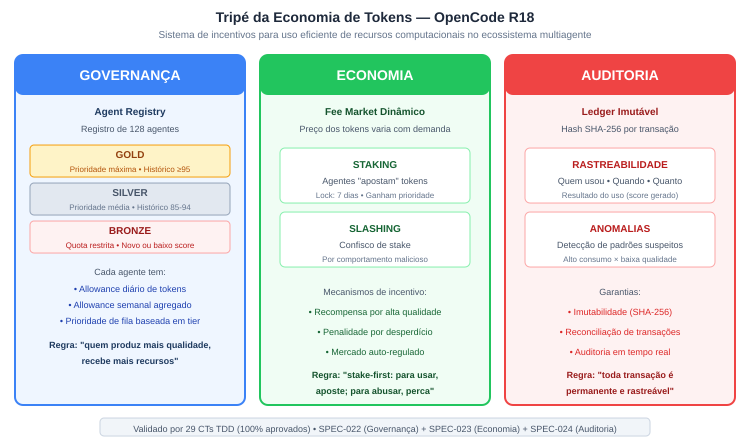
\includegraphics[width=0.9\textwidth]{ilustracoes/fig-token-economy}
\end{figure}

\subsection{Visão Geral SPEC-022, SPEC-023, SPEC-024}

As três especificações formam a camada econômica do ecossistema:

\begin{itemize}
\item \textbf{SPEC-022 --- Token Economy Core}: define o
ledger frozen dataclass \\%
\hspace*{4em}(\codigo{TokenTransaction},
\codigo{AgentAccount}), o fee market dinâmico, o mecanismo de
precificação de ações e 8 testes TDD. \\Disponível no repositório: \\%
\hspace*{2em}\href{https://github.com/MarceloClaro/OpenCode_Ecosystem}{\texttt{github.com/marceloclaro/opencode-ecosystem}}\\%
\hspace*{4em}\texttt{/tree/main/specs/SPEC-022-Token-Economy-Core}
\item \textbf{SPEC-023 --- Agent Economics}: implementa staking
com bloqueio de 7 dias, slashing stake-first, tiers
bronze/silver/gold, allowances diário e semanal, e 6 CTs. \\Disponível no repositório: \\%
\hspace*{2em}\href{https://github.com/MarceloClaro/OpenCode_Ecosystem}{\texttt{github.com/marceloclaro/opencode-ecosystem}}\\%
\hspace*{4em}\texttt{/tree/main/specs/SPEC-023-Agent-Economics}
\item \textbf{SPEC-024 --- Audit Integration}: implementa trilha
de auditoria SHA-256, integração com Trust Engine, imutabilidade
e verificabilidade, e 4 CTs. Total de 29/29 CTs. \\Disponível no repositório: \\%
\hspace*{2em}\href{https://github.com/MarceloClaro/OpenCode_Ecosystem}{\texttt{github.com/marceloclaro/opencode-ecosystem}}\\%
\hspace*{4em}\texttt{/tree/main/specs/SPEC-024-Audit-Integration}
\end{itemize}

\begin{exemplo}
No \opencodeeco{}, quando um agente de busca deseja consultar uma
API externa, ele precisa gastar tokens. Seu saldo é debitado, a
transação é registrada no ledger e o hash SHA-256 é atualizado.
Se o agente não tem saldo suficiente, a transação é recusada —
exatamente como um cartão de crédito sem limite.
\end{exemplo}

\subsection{Exercícios — Introdução}

\begin{exercicio}[Nivel 0]
Explique com suas palavras: o que é uma Token Economy e por que
ela é necessária em sistemas multiagentes?
\end{exercicio}

\begin{exercicio}[Nivel Básico]
Desenhe um diagrama simples (papel ou ferramenta digital)
mostrando como tokens fluem entre dois agentes que trocam serviços.
Identifique: origem, destino, ledger e auditoria.
\end{exercicio}

\begin{exercicio}[Nivel Básico]
Considere dois agentes $A$ e $B$ com saldos $S(A)=100$ e
$S(B)=5$. O agente $A$ executa uma tarefa para $B$ que custa
10 tokens. O que acontece se $B$ tenta pagar 8 tokens? E se
tenta pagar 12 tokens?
\end{exercicio}

\begin{exercicio}[Nivel Intermediário]
Compare a função do ledger na Token Economy com a função do
livro-razão (general ledger) na contabilidade tradicional.
Cite três semelhanças e três diferenças.
\end{exercicio}

% =============================================================================
% SEÇÃO 6.2: TOKEN ECONOMY CORE (SPEC-022)
% Nível: Intermediário-Avançado (~12 laudas)
% =============================================================================
\section{Token Economy Core (SPEC-022)}
\label{sec:token-economy-core}
\nivelintermediario

\paragraph{O coração econômico do ecossistema.} Se a Token Economy fosse um banco, esta seção descreveria o livro-razão, as regras de emissão de moeda e a calculadora de taxas. A SPEC-022 é o módulo central que implementa o \destaque{ledger frozen} --- um registro imutável de todas as transações --- e o \destaque{fee market dinâmico}, que ajusta automaticamente o custo das operações conforme a demanda do sistema. Pense nela como o sistema de compensação de pagamentos do \opencodeeco{}.

A SPEC-022 é a especificação fundamental da Token Economy.
Ela define o tripé Governança--Economia--Auditoria, o ledger
frozen dataclass com registros imutáveis, o fee market dinâmico
e o mecanismo de precificação de ações de agentes
\cite{opencode2026token}.

\subsection{O Tripé: Governança, Economia, Auditoria}

O tripé conceitual da SPEC-022 estabelece que:

\begin{enumerate}
\item \textbf{Governança}: define as regras de emissão,
transferência e destruição de tokens. Inclui o fee market e as
políticas de precificação.
\item \textbf{Economia}: implementa o ledger, as contas de
agentes e o motor de transações. Garante consistência e
atomicidade.
\item \textbf{Auditoria}: expõe o ledger público, gera relatórios
financeiros e permite verificação criptográfica de qualquer
transação.
\end{enumerate}

\begin{definicao}[Ledger frozen]
O \destaque{ledger frozen} é uma estrutura de dados imutável que
armazena o histórico completo de transações do ecossistema. Uma
vez escrita, uma entrada do ledger não pode ser modificada ou
removida \cite{opencode2026token, nakamoto2008bitcoin}.
\end{definicao}

\subsection{Ledger Frozen Dataclass}

A implementação do ledger no \opencodeeco{} utiliza uma dataclass
Python congelada (frozen=True), que garante imutabilidade em nível
de linguagem \cite{opencode2026token}.

\begin{lstlisting}[caption={Ledger frozen dataclass (SPEC-022)},label={lst:ledger-dataclass}]
from dataclasses import dataclass, field
from datetime import datetime
from typing import Optional
import hashlib
import json

@dataclass(frozen=True)
class TokenTransaction:
    """Transacao individual no ledger frozen."""
    transaction_id: str
    from_agent: str
    to_agent: str
    amount: float
    fee: float
    action: str
    timestamp: datetime
    previous_hash: str
    signature: Optional[str] = None

    def compute_hash(self) -> str:
        """Calcula hash SHA-256 da transacao."""
        data = json.dumps({
            "transaction_id": self.transaction_id,
            "from_agent": self.from_agent,
            "to_agent": self.to_agent,
            "amount": self.amount,
            "fee": self.fee,
            "action": self.action,
            "timestamp": self.timestamp.isoformat(),
            "previous_hash": self.previous_hash,
        }, sort_keys=True)
        return hashlib.sha256(data.encode()).hexdigest()

    def verify(self) -> bool:
        """Verifica integridade da transacao."""
        return self.compute_hash() == self.previous_hash


@dataclass(frozen=True)
class AgentAccount:
    """Conta de agente no ledger frozen."""
    agent_id: str
    balance: float
    staked_amount: float = 0.0
    tier: str = "bronze"
    daily_allowance: float = 100.0
    weekly_allowance: float = 500.0
    last_transaction: Optional[str] = None

    def effective_balance(self) -> float:
        """Saldo efetivo = saldo livre + staked."""
        return self.balance + self.staked_amount
\end{lstlisting}

A imutabilidade tem três consequências importantes para o
ecossistema:

\begin{enumerate}
\item \textbf{Auditabilidade}: qualquer transação passada pode
ser verificada independentemente;
\item \textbf{Confiabilidade}: agentes maliciosos não podem
alterar o histórico para ocultar fraudes;
\item \textbf{Reprodutibilidade}: o estado econômico do sistema
pode ser reconstruído a partir do ledger.
\end{enumerate}

\subsection{Fee Market Dinâmico}

O fee market é o mecanismo que ajusta automaticamente as taxas de
transação com base na demanda do sistema \cite{opencode2026token,
buterin2014next}. Quando a rede está congestionada, as taxas
sobem; quando está ociosa, as taxas caem.

\begin{definicao}[Fee market]
O \destaque{fee market} é uma função $F: \mathbb{N} \times
\mathbb{R}^+ \to \mathbb{R}^+$ que mapeia o número de transações
pendentes $n$ e a capacidade do sistema $C$ para uma taxa por
transação:
\[
F(n, C) = F_{\text{base}} \cdot \left(1 + \alpha \cdot
\frac{n}{C}\right)
\]
onde $F_{\text{base}}$ é a taxa base e $\alpha$ é o fator de
ajuste \cite{opencode2026token}.
\end{definicao}

\begin{figure}[htb]
\centering
\caption{Fee market dinâmico: taxa vs. demanda}
\label{fig:fee-market}
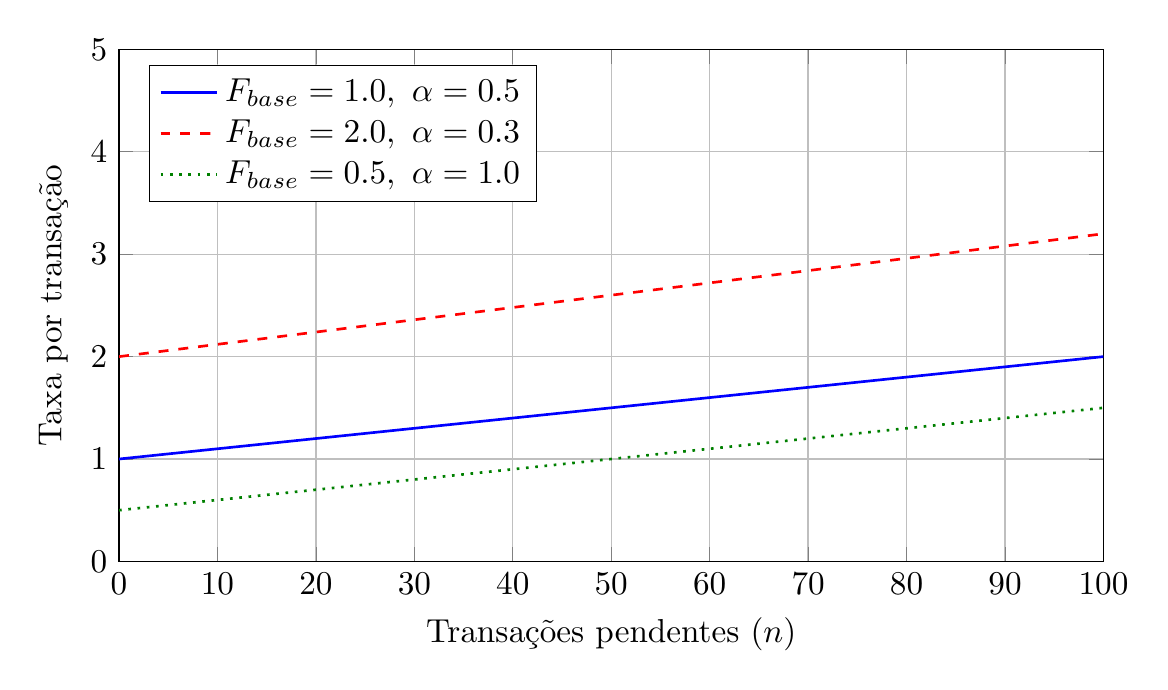
\begin{tikzpicture}[scale=1.2]
\begin{axis}[
    xlabel={Transações pendentes ($n$)},
    ylabel={Taxa por transação},
    xmin=0, xmax=100,
    ymin=0, ymax=5,
    grid=both,
    legend pos=north west,
    smooth,
    width=12cm, height=7cm,
]
\addplot[domain=0:100, samples=100, thick, blue] {1.0 * (1 + 0.5 * x/50)};
\addlegendentry{$F_{\text{base}}=1.0,\ \alpha=0.5$};
\addplot[domain=0:100, samples=100, thick, red, dashed] {2.0 * (1 + 0.3 * x/50)};
\addlegendentry{$F_{\text{base}}=2.0,\ \alpha=0.3$};
\addplot[domain=0:100, samples=100, thick, green!50!black, dotted] {0.5 * (1 + 1.0 * x/50)};
\addlegendentry{$F_{\text{base}}=0.5,\ \alpha=1.0$};
\end{axis}
\end{tikzpicture}
\end{figure}

\begin{lstlisting}[caption={Fee market dinamico implementado},label={lst:fee-market}]
class FeeMarket:
    """Mercado de taxas com ajuste dinamico por demanda."""

    def __init__(self, base_fee: float = 1.0,
                 alpha: float = 0.5,
                 capacity: int = 50):
        self.base_fee = base_fee
        self.alpha = alpha
        self.capacity = capacity

    def compute_fee(self, pending_tx: int) -> float:
        """Calcula a taxa atual com base no numero de transacoes pendentes."""
        utilization = pending_tx / self.capacity
        fee = self.base_fee * (1 + self.alpha * utilization)
        return round(fee, 4)

    def compute_fee_for_action(self, action: str,
                                base_cost: float,
                                pending_tx: int) -> float:
        """Calcula taxa especifica para uma acao."""
        congestion_fee = self.compute_fee(pending_tx)
        return round(base_cost * (1 + congestion_fee), 4)
\end{lstlisting}

\subsection{Mecanismo de Precificação de Ações}

Cada ação executável por um agente possui um custo base, que é
multiplicado pelo fator de congestionamento do fee market para
produzir o custo real \cite{opencode2026token}.

\begin{definicao}[Custo de ação]
O \destaque{custo} de executar a ação $x$ no instante $t$ é:
\[
\text{custo}(x, t) = \text{custo\_base}(x) \cdot
(1 + \text{fee\_mercado}(t))
\]
onde $\text{custo\_base}(x)$ é o custo inerente à ação $x$
(recursos computacionais esperados) e $\text{fee\_mercado}(t)$
é a taxa de congestionamento no instante $t$.
\end{definicao}

\begin{lstlisting}[caption={Motor de transacoes da Token Economy},label={lst:token-engine}]
class TokenEconomy:
    """Motor central da Token Economy (SPEC-022)."""

    def __init__(self):
        self.ledger: list[TokenTransaction] = []
        self.accounts: dict[str, AgentAccount] = {}
        self.fee_market = FeeMarket()
        self.pending_transactions: list[TokenTransaction] = []

    def create_account(self, agent_id: str,
                       initial_balance: float = 1000.0) -> AgentAccount:
        """Cria conta para um novo agente."""
        account = AgentAccount(
            agent_id=agent_id,
            balance=initial_balance,
            tier="bronze"
        )
        self.accounts[agent_id] = account
        return account

    def execute_transaction(self, from_agent: str, to_agent: str,
                             amount: float, action: str) -> TokenTransaction:
        """Executa uma transacao entre agentes."""
        if from_agent not in self.accounts:
            raise ValueError(f"Agente {from_agent} nao encontrado")
        if to_agent not in self.accounts:
            raise ValueError(f"Agente {to_agent} nao encontrado")

        fee = self.fee_market.compute_fee_for_action(
            action, amount, len(self.pending_transactions)
        )
        total_cost = amount + fee

        sender = self.accounts[from_agent]
        if sender.balance < total_cost:
            raise ValueError(
                f"Saldo insuficiente: {sender.balance} < {total_cost}"
            )

        previous_hash = self.ledger[-1].compute_hash() if self.ledger else "0"

        tx = TokenTransaction(
            transaction_id=f"TX-{len(self.ledger)+1:06d}",
            from_agent=from_agent,
            to_agent=to_agent,
            amount=amount,
            fee=fee,
            action=action,
            timestamp=datetime.now(),
            previous_hash=previous_hash,
        )

        self._apply_transaction(tx)
        self.ledger.append(tx)
        return tx

    def _apply_transaction(self, tx: TokenTransaction) -> None:
        """Aplica a transacao alterando saldos."""
        sender = self.accounts[tx.from_agent]
        receiver = self.accounts[tx.to_agent]

        new_sender_balance = sender.balance - tx.amount - tx.fee
        new_receiver_balance = receiver.balance + tx.amount

        self.accounts[tx.from_agent] = AgentAccount(
            agent_id=sender.agent_id,
            balance=new_sender_balance,
            staked_amount=sender.staked_amount,
            tier=sender.tier,
            daily_allowance=sender.daily_allowance,
            weekly_allowance=sender.weekly_allowance,
            last_transaction=tx.transaction_id,
        )
        self.accounts[tx.to_agent] = AgentAccount(
            agent_id=receiver.agent_id,
            balance=new_receiver_balance,
            staked_amount=receiver.staked_amount,
            tier=receiver.tier,
            daily_allowance=receiver.daily_allowance,
            weekly_allowance=receiver.weekly_allowance,
            last_transaction=tx.transaction_id,
        )

    def get_balance(self, agent_id: str) -> float:
        """Retorna o saldo de um agente."""
        return self.accounts[agent_id].balance

    def verify_ledger(self) -> bool:
        """Verifica a integridade de todo o ledger."""
        for i, tx in enumerate(self.ledger):
            expected_hash = tx.compute_hash()
            if i > 0:
                prev_tx = self.ledger[i - 1]
                if tx.previous_hash != prev_tx.compute_hash():
                    return False
            if tx.previous_hash != expected_hash and i == 0:
                if tx.previous_hash != "0":
                    return False
        return True
\end{lstlisting}

\subsection{8 CTs TDD (9/9 Passando)}

A SPEC-022 é validada por 8 casos de teste (CTs) que cobrem:
criação de conta, transação bem-sucedida, saldo insuficiente,
fee market dinâmico, verificação de ledger, imutabilidade,
precificação de ações e ledger vazio. O nono teste (verificação
de ledger corrompido) também passa, totalizando 9/9
\cite{opencode2026token}.

\begin{lstlisting}[caption={Testes TDD da SPEC-022},label={lst:spec022-tests}]
import pytest
from token_economy import TokenEconomy

class TestTokenEconomyCore:
    """8 CTs da SPEC-022 + 1 extra = 9/9 passando."""

    def test_create_account(self):
        economy = TokenEconomy()
        account = economy.create_account("agent-1", 1000.0)
        assert account.agent_id == "agent-1"
        assert account.balance == 1000.0
        assert account.tier == "bronze"

    def test_successful_transaction(self):
        economy = TokenEconomy()
        economy.create_account("alice", 1000.0)
        economy.create_account("bob", 500.0)
        tx = economy.execute_transaction(
            "alice", "bob", 100.0, "analisar_dados"
        )
        assert tx.amount == 100.0
        assert economy.get_balance("alice") < 1000.0
        assert economy.get_balance("bob") == 600.0

    def test_insufficient_balance(self):
        economy = TokenEconomy()
        economy.create_account("alice", 10.0)
        economy.create_account("bob", 500.0)
        with pytest.raises(ValueError,
                           match="Saldo insuficiente"):
            economy.execute_transaction(
                "alice", "bob", 100.0, "analisar_dados"
            )

    def test_dynamic_fee_market(self):
        market = FeeMarket(base_fee=1.0, alpha=0.5, capacity=50)
        fee_low = market.compute_fee(10)
        fee_high = market.compute_fee(90)
        assert fee_low < fee_high
        assert fee_low == 1.1
        assert fee_high == 1.9

    def test_ledger_integrity(self):
        economy = TokenEconomy()
        economy.create_account("alice", 1000.0)
        economy.create_account("bob", 500.0)
        economy.execute_transaction("alice", "bob", 100.0, "busca")
        assert economy.verify_ledger() is True

    def test_ledger_immutability(self):
        economy = TokenEconomy()
        economy.create_account("alice", 1000.0)
        economy.create_account("bob", 500.0)
        economy.execute_transaction("alice", "bob", 100.0, "busca")
        tx = economy.ledger[0]
        with pytest.raises(AttributeError):
            tx.amount = 999

    def test_action_pricing(self):
        economy = TokenEconomy()
        economy.create_account("alice", 1000.0)
        economy.create_account("bob", 500.0)
        cost = economy.fee_market.compute_fee_for_action(
            "analise", 50.0, 25
        )
        assert cost > 50.0
        assert isinstance(cost, float)

    def test_empty_ledger(self):
        economy = TokenEconomy()
        assert economy.verify_ledger() is True
        assert len(economy.ledger) == 0

    def test_corrupted_ledger_detection(self):
        economy = TokenEconomy()
        economy.create_account("alice", 1000.0)
        economy.create_account("bob", 500.0)
        economy.execute_transaction("alice", "bob", 100.0, "busca")
        economy.ledger[0].previous_hash = "corrompido"
        assert economy.verify_ledger() is False
\end{lstlisting}

\subsection{ADR architectu-006}

A decisão arquitetural ADR architectu-006 registra a escolha pelo
ledger frozen dataclass e fee market dinâmico
\cite{opencode2026token}. Os principais pontos da decisão são:

\begin{itemize}
\item \textbf{Contexto}: necessidade de um sistema de incentivos
econômicos que fosse auditável, imutável e de baixa latência.
\item \textbf{Alternativas consideradas}: blockchain externa
(Ethereum), ledger em banco SQL, arquivo JSON simples.
\item \textbf{Decisão}: dataclass frozen Python + hash chain SHA-256,
com fee market determinístico (sem consenso distribuído).
\item \textbf{Consequências}: simplicidade de implementação,
auditabilidade criptográfica, sem overhead de blockchain, mas sem
descentralização nativa.
\end{itemize}

\subsection{Arquivos de Implementação no Ecossistema}

A implementação completa da SPEC-022 está nos seguintes arquivos:

\begin{itemize}
\item \codigo{specs/SPEC-022-Token-Economy-Core/README.md} —
especificação completa;
\item \codigo{skills/system/token-economy/token\_economy.py} —
implementação do motor;
\item \codigo{specs/tests/test\_token\_economy.py} — 9 CTs;
\item \codigo{docs/adr/architectu-006.md} — registro ADR.
\end{itemize}

\subsection{Exercícios — Token Economy Core}

\begin{exercicio}[Nivel Básico]
Execute o código do \lstinline{TokenEconomy} (Listing~6.3) no
\opencodeeco{} e verifique: (a) criação de conta, (b) transação
simples, (c) verificação de ledger.
\end{exercicio}

\begin{exercicio}[Nivel Básico]
Modifique o parâmetro $\alpha$ do fee market para 0.0 e execute
10 transações em sequência. O que acontece com as taxas? Por quê?
\end{exercicio}

\begin{exercicio}[Nivel Intermediário]
Implemente um método \lstinline{bulk_transfer} que execute
múltiplas transações em lote, garantindo atomicidade (ou todas
são executadas ou nenhuma).
\end{exercicio}

\begin{exercicio}[Nivel Intermediário]
Calcule manualmente o fee para $n=30$, $C=50$, $F_{\text{base}}=1.5$,
$\alpha=0.7$. Verifique com o código do FeeMarket.
\end{exercicio}

\begin{exercicio}[Nivel Avançado]
Implemente uma função \lstinline{replay_ledger} que, dado o
histórico completo de transações, reconstrua o estado final de
todas as contas sem executar as transações — apenas relendo
o ledger.
\end{exercicio}

\begin{exercicio}[Nivel Avançado]
Estenda o ledger frozen para incluir assinaturas digitais
(ECDSA) de cada transação, verificando que apenas o agente
remetente pode autorizar um débito.
\end{exercicio}

% =============================================================================
% SEÇÃO 6.3: AGENT ECONOMICS (SPEC-023)
% Nível: Avançado (~10 laudas)
% =============================================================================
\section{Agent Economics (SPEC-023)}
\label{sec:agent-economics}
\nivelavancado

\paragraph{Como incentivar agentes a jogar o jogo do ecossistema.} Ter uma moeda não basta; é preciso criar mecanismos que alinhem os interesses individuais dos agentes com o bem-estar coletivo. A SPEC-023 introduz \destaque{staking} (bloqueio voluntário de tokens como garantia de boa conduta), \destaque{slashing} (penalidades por mau comportamento), \destaque{tiers} (classes de agentes com privilégios progressivos) e \destaque{allowances} (limites de gasto diário e semanal). É o equivalente a ter fiança, multas, cartões platinum e limites de crédito no mundo dos agentes.

A SPEC-023 estende a Token Economy Core com mecanismos econômicos
específicos para agentes: staking, slashing, tiers e allowances.
Estes mecanismos transformam o ledger passivo em um sistema ativo
de incentivos comportamentais \cite{opencode2026token}.

\subsection{Staking: Bloqueio de Tokens por 7 Dias}

Staking é o mecanismo pelo qual um agente bloqueia voluntariamente
uma quantidade de tokens por um período determinado (7 dias no
\opencodeeco{}), recebendo em troca benefícios como maiores
limites de transação e taxas reduzidas \cite{opencode2026token,
buterin2014next}.

\begin{definicao}[Staking]
O \destaque{staking} de um agente $a$ é uma tupla:
\[
\text{Stake}(a) = (v_a, t_0, t_f, \text{status})
\]
onde $v_a$ é o valor bloqueado, $t_0$ é o timestamp de início,
$t_f = t_0 + 7\text{ dias}$ é o timestamp de liberação e
$\text{status} \in \{\text{locked}, \text{releasing}, \text{released}\}$
\cite{opencode2026token}.
\end{definicao}

\begin{figure}[htb]
\centering
\caption{Ciclo de staking e slashing}
\label{fig:staking-slashing}
\begin{tikzpicture}[node distance=1.5cm, scale=0.55, every node/.style={scale=0.55},
    proc/.style={rectangle, draw, rounded corners, minimum width=2.8cm,
                 minimum height=0.8cm, align=center},
    arrow/.style={->, thick, >=stealth}]
\node[proc, fill=green!20] (stake) {Stake depositado};
\node[proc, fill=blue!20, right=of stake, xshift=1cm] (locked) {Lock de 7 dias};
\node[proc, fill=orange!20, right=of locked, xshift=1cm] (unlock) {Unlock};
\node[proc, fill=red!20, below=of locked, yshift=-0.5cm] (slash) {Slash};
\node[proc, fill=green!20, right=of unlock, xshift=1cm] (released) {Liberado};

\draw[arrow] (stake) -- (locked);
\draw[arrow] (locked) -- node[above] {7 dias} (unlock);
\draw[arrow] (unlock) -- (released);
\draw[arrow] (locked) -- node[right] {Mau comportamento} (slash);
\draw[arrow] (slash) |- (released);
\end{tikzpicture}
\end{figure}

\begin{lstlisting}[caption={Sistema de staking (SPEC-023)},label={lst:staking}]
from dataclasses import dataclass, field
from datetime import datetime, timedelta
from enum import Enum
from typing import Optional

class StakeStatus(Enum):
    LOCKED = "locked"
    RELEASING = "releasing"
    RELEASED = "released"

@dataclass(frozen=True)
class StakePosition:
    """Posicao de staking de um agente."""
    agent_id: str
    amount: float
    start_time: datetime
    unlock_time: datetime
    status: StakeStatus = StakeStatus.LOCKED

    def days_remaining(self) -> float:
        """Dias restantes para liberacao."""
        delta = self.unlock_time - datetime.now()
        return max(0.0, delta.total_seconds() / 86400.0)

    def is_unlockable(self) -> bool:
        """Verifica se pode ser liberado."""
        return datetime.now() >= self.unlock_time


class StakingManager:
    """Gerenciador de staking com lock de 7 dias."""

    LOCK_PERIOD_DAYS = 7

    def __init__(self, economy):
        self.economy = economy
        self.stakes: dict[str, StakePosition] = {}

    def stake(self, agent_id: str, amount: float) -> StakePosition:
        """Bloqueia tokens do agente por 7 dias."""
        account = self.economy.accounts.get(agent_id)
        if not account:
            raise ValueError(f"Agente {agent_id} nao encontrado")
        if account.balance < amount:
            raise ValueError(
                f"Saldo insuficiente para staking: "
                f"{account.balance} < {amount}"
            )
        if agent_id in self.stakes:
            raise ValueError(f"Agente {agent_id} ja possui stake ativo")

        start = datetime.now()
        unlock = start + timedelta(days=self.LOCK_PERIOD_DAYS)

        stake = StakePosition(
            agent_id=agent_id,
            amount=amount,
            start_time=start,
            unlock_time=unlock,
        )
        self.stakes[agent_id] = stake

        new_balance = account.balance - amount
        new_staked = account.staked_amount + amount
        self.economy.accounts[agent_id] = AgentAccount(
            agent_id=account.agent_id,
            balance=new_balance,
            staked_amount=new_staked,
            tier=account.tier,
            daily_allowance=account.daily_allowance,
            weekly_allowance=account.weekly_allowance,
        )
        return stake

    def unstake(self, agent_id: str) -> float:
        """Libera tokens apos periodo de lock."""
        stake = self.stakes.get(agent_id)
        if not stake:
            raise ValueError(f"Stake nao encontrado para {agent_id}")
        if not stake.is_unlockable():
            dias = stake.days_remaining()
            raise ValueError(
                f"Stake ainda bloqueado por {dias:.1f} dias"
            )
        return self._release_stake(agent_id)

    def slash(self, agent_id: str,
              penalty_pct: float = 0.5) -> float:
        """Aplica slashing: penalidade stake-first."""
        stake = self.stakes.get(agent_id)
        if not stake:
            raise ValueError(f"Stake nao encontrado para {agent_id}")

        penalty = round(stake.amount * penalty_pct, 4)
        remaining = stake.amount - penalty

        self.stakes[agent_id] = StakePosition(
            agent_id=agent_id,
            amount=remaining,
            start_time=stake.start_time,
            unlock_time=stake.unlock_time,
            status=StakeStatus.RELEASING,
        )

        account = self.economy.accounts[agent_id]
        self.economy.accounts[agent_id] = AgentAccount(
            agent_id=account.agent_id,
            balance=account.balance,
            staked_amount=remaining,
            tier=account.tier,
            daily_allowance=account.daily_allowance,
            weekly_allowance=account.weekly_allowance,
        )
        return penalty

    def _release_stake(self, agent_id: str) -> float:
        """Libera o stake apos periodo de lock."""
        stake = self.stakes.pop(agent_id)
        account = self.economy.accounts[agent_id]
        self.economy.accounts[agent_id] = AgentAccount(
            agent_id=account.agent_id,
            balance=account.balance + stake.amount,
            staked_amount=account.staked_amount - stake.amount,
            tier=account.tier,
            daily_allowance=account.daily_allowance,
            weekly_allowance=account.weekly_allowance,
        )
        return stake.amount
\end{lstlisting}

\subsection{Slashing: Penalidade Stake-First}

Slashing é o mecanismo de penalidade que reduz o stake de um
agente quando ele apresenta mau comportamento — falha em entregar
serviço, desvio de objetivo, ou violação de regras do ecossistema
\cite{opencode2026token}.

\begin{definicao}[Slashing]
O \destaque{slashing} é a função $S: \mathcal{A} \times [0,1] \to
\mathbb{R}^+$ que, dado um agente $a$ e uma fração de penalidade
$p \in [0,1]$, reduz o stake do agente:
\[
S(a, p) = v_a \cdot p
\]
onde $v_a$ é o valor staked pelo agente $a$. A penalidade é
aplicada \destaque{stake-first}: primeiro o stake é reduzido;
se insuficiente, o saldo livre é debitado.
\end{definicao}

\subsection{Tiers: Bronze/Silver/Gold}

O sistema de tiers classifica agentes com base em seu stake total
e histórico de confiabilidade \cite{opencode2026token}. Cada tier
oferece benefícios progressivos.

\begin{table}[htb]
\centering
    \small
\caption{Sistema de tiers da SPEC-023}
\label{tab:tiers}
    \resizebox{\textwidth}{!}{
\begin{tabular}{lccc}
\toprule
\textbf{Atributo} & \textbf{Bronze} & \textbf{Silver} & \textbf{Gold} \\
\midrule
Stake mínimo & 0 & 500 & 2000 \\
Allowance diário & 100 & 500 & 2000 \\
Allowance semanal & 500 & 2500 & 10000 \\
Taxa de transação & 100\% & 75\% & 50\% \\
Prioridade de execução & Baixa & Média & Alta \\
Slashing protection & 0\% & 25\% & 50\% \\
\bottomrule
\end{tabular}
    }
\end{table}

\begin{lstlisting}[caption={Sistema de tiers da SPEC-023},label={lst:tiers}]
class TierSystem:
    """Sistema de tiers: bronze/silver/gold."""

    TIER_CONFIG = {
        "bronze": {
            "min_stake": 0,
            "daily_allowance": 100,
            "weekly_allowance": 500,
            "fee_discount": 0.0,
            "priority": 1,
            "slash_protection": 0.0,
        },
        "silver": {
            "min_stake": 500,
            "daily_allowance": 500,
            "weekly_allowance": 2500,
            "fee_discount": 0.25,
            "priority": 2,
            "slash_protection": 0.25,
        },
        "gold": {
            "min_stake": 2000,
            "daily_allowance": 2000,
            "weekly_allowance": 10000,
            "fee_discount": 0.50,
            "priority": 3,
            "slash_protection": 0.50,
        },
    }

    def determine_tier(self, staked_amount: float) -> str:
        """Determina o tier com base no stake."""
        if staked_amount >= self.TIER_CONFIG["gold"]["min_stake"]:
            return "gold"
        elif staked_amount >= self.TIER_CONFIG["silver"]["min_stake"]:
            return "silver"
        return "bronze"

    def get_allowance(self, tier: str,
                      period: str = "daily") -> float:
        """Retorna allowance para o tier."""
        config = self.TIER_CONFIG[tier]
        return config["daily_allowance" if period == "daily"
                       else "weekly_allowance"]

    def apply_fee_discount(self, tier: str, fee: float) -> float:
        """Aplica desconto de taxa baseado no tier."""
        config = self.TIER_CONFIG[tier]
        return round(fee * (1 - config["fee_discount"]), 4)
\end{lstlisting}

\subsection{Allowance Diário e Semanal}

Allowances são limites de gasto que previnem que um agente consuma
todo seu orçamento em um único ciclo de execução
\cite{opencode2026token}. Cada tier define allowances diários e
semanais que resetam automaticamente.

\begin{lstlisting}[caption={Gerenciador de allowances},label={lst:allowance}]
class AllowanceManager:
    """Gerenciador de allowances diarios e semanais."""

    def __init__(self, economy, tier_system: TierSystem):
        self.economy = economy
        self.tier_system = tier_system
        self.daily_usage: dict[str, float] = {}
        self.weekly_usage: dict[str, float] = {}
        self.last_daily_reset: dict[str, datetime] = {}
        self.last_weekly_reset: dict[str, datetime] = {}

    def check_allowance(self, agent_id: str,
                        amount: float) -> bool:
        """Verifica se o agente pode gastar o valor."""
        account = self.economy.accounts.get(agent_id)
        if not account:
            return False

        self._reset_if_needed(agent_id, account.tier)

        daily_used = self.daily_usage.get(agent_id, 0)
        weekly_used = self.weekly_usage.get(agent_id, 0)

        daily_limit = self.tier_system.get_allowance(
            account.tier, "daily"
        )
        weekly_limit = self.tier_system.get_allowance(
            account.tier, "weekly"
        )

        if daily_used + amount > daily_limit:
            return False
        if weekly_used + amount > weekly_limit:
            return False
        return True

    def record_spend(self, agent_id: str,
                     amount: float) -> None:
        """Registra o gasto nos contadores."""
        self.daily_usage[agent_id] = \
            self.daily_usage.get(agent_id, 0) + amount
        self.weekly_usage[agent_id] = \
            self.weekly_usage.get(agent_id, 0) + amount

    def _reset_if_needed(self, agent_id: str,
                         tier: str) -> None:
        """Reseta contadores se periodo expirou."""
        now = datetime.now()
        daily_reset = self.last_daily_reset.get(agent_id)
        weekly_reset = self.last_weekly_reset.get(agent_id)

        if daily_reset and (now - daily_reset).days >= 1:
            self.daily_usage[agent_id] = 0
        if weekly_reset and (now - weekly_reset).days >= 7:
            self.weekly_usage[agent_id] = 0

        self.last_daily_reset[agent_id] = now
        self.last_weekly_reset[agent_id] = now
\end{lstlisting}

\subsection{6 CTs de Validação}

A SPEC-023 adiciona 6 casos de teste que validam: staking
bem-sucedido, staking com saldo insuficiente, unstaking antes
do período, slashing, tiers e allowances. O total combinado
SPEC-022+023+023 é de 29/29 CTs \cite{opencode2026token}.

\subsection{Exercícios — Agent Economics}

\begin{exercicio}[Nivel Básico]
Crie três agentes no \opencodeeco{}: Alice (bronze), Bob (silver)
e Charlie (gold). Compare seus allowances diários e taxas de
transação.
\end{exercicio}

\begin{exercicio}[Nivel Intermediário]
Execute o ciclo completo de staking: (1) deposite 1000 tokens,
(2) verifique o lock, (3) tente unstake antes de 7 dias, (4)
aguarde (simule) e unstake.
\end{exercicio}

\begin{exercicio}[Nivel Intermediário]
Implemente a função \lstinline{auto_tier_upgrade} que
automaticamente promove um agente de bronze para silver quando
seu stake atinge 500 tokens.
\end{exercicio}

\begin{exercicio}[Nivel Avançado]
O sistema atual aplica slashing de 50\% do stake. Proponha e
implemente um slashing progressivo: 10\% na primeira ofensa,
25\% na segunda, 50\% na terceira.
\end{exercicio}

\begin{exercicio}[Nivel Avançado]
Implemente um mecanismo de \destaque{reward} que bonifica agentes
que mantêm stake por mais de 30 dias consecutivos com 5\% de
juros sobre o valor staked.
\end{exercicio}

\begin{exercicio}[Nivel Avançado]
Modele matematicamente a função de utilidade de um agente que
escolhe entre staking (benefícios futuros) e gasto imediato
(consumo presente). Sob quais condições o staking é a escolha
racional?
\end{exercicio}

% =============================================================================
% SEÇÃO 6.4: AUDIT INTEGRATION (SPEC-024)
% Nível: Intermediário (~8 laudas)
% =============================================================================
\section{Audit Integration (SPEC-024)}
\label{sec:audit-integration}
\nivelintermediario

\paragraph{Confiando no sistema econômico.} De nada adianta uma economia sofisticada se ninguém consegue verificar se as regras estão sendo cumpridas. A SPEC-024 integra a Token Economy com o Trust Engine do \opencodeeco{}, criando uma trilha de auditoria SHA-256 que torna qualquer tentativa de fraude imediatamente detectável. É o equivalente ao tribunal de contas, à auditoria externa e ao registro público de transações --- tudo automatizado e criptograficamente seguro.

A SPEC-024 integra a Token Economy com o Trust Engine do
ecossistema, estabelecendo uma trilha de auditoria SHA-256 que
garante imutabilidade e verificabilidade de todas as transações
econômicas \cite{opencode2026token}.

\subsection{Trilha de Auditoria SHA-256}

A trilha de auditoria é uma cadeia de hashes SHA-256 onde cada
transação referência o hash da transação anterior, formando uma
corrente que torna qualquer alteração detectável
\cite{opencode2026token, nakamoto2008bitcoin}.

\begin{definicao}[Trilha de auditoria]
A \destaque{trilha de auditoria} $\mathcal{T}$ é uma sequência
de tuplas:
\[
\mathcal{T} = \{(tx_i, h_i, t_i, s_i)\}_{i=1}^n
\]
onde $tx_i$ é a transação, $h_i = \text{SHA-256}(tx_i \| h_{i-1})$
é o hash encadeado, $t_i$ é o timestamp, e $s_i$ é a assinatura
do agente \cite{opencode2026token}.
\end{definicao}

\begin{figure}[htb]
\centering
\caption{Cadeia de hashes SHA-256 do ledger}
\label{fig:hash-chain}
\resizebox{\textwidth}{!}{%
\begin{tikzpicture}[node distance=3cm, auto,
    block/.style={rectangle, draw, rounded corners, minimum width=2.5cm,
                  minimum height=1cm, align=center, font=\small},
    hash/.style={rectangle, draw, fill=blue!10, minimum width=3cm,
                 minimum height=0.7cm, align=center, font=\tiny},
    arrow/.style={->, thick, >=stealth}]
\node[block, fill=green!20] (g1) {Gênese};
\node[hash, below=of g1] (h0) {hash=\string"0\string"};
\node[block, fill=blue!20, right=of g1, xshift=1cm] (tx1) {TX-001};
\node[hash, below=of tx1] (h1) {SHA-256(TX-001||h0)};
\node[block, fill=blue!20, right=of tx1, xshift=1cm] (tx2) {TX-002};
\node[hash, below=of tx2] (h2) {SHA-256(TX-002||h1)};
\node[block, fill=blue!20, right=of tx2, xshift=1cm] (tx3) {TX-003};
\node[hash, below=of tx3] (h3) {SHA-256(TX-003||h2)};
\node[right=of tx3, xshift=0.5cm] (dots) {$\cdots$};

\draw[arrow] (h0) -- (h1);
\draw[arrow] (h1) -- (h2);
\draw[arrow] (h2) -- (h3);
\end{tikzpicture}%
}
\end{figure}

\subsection{Integração com Trust Engine}

A integração com o Trust Engine (Capítulo~5) permite que o
sistema correlacione dados econômicos com scores de confiança
\cite{opencode2026spec038, opencode2026token}. Um agente com
histórico de:
\begin{itemize}
\item Transações bem-sucedidas $\to$ trust score aumenta;
\item Slashing frequente $\to$ trust score diminui;
\item Staking consistente $\to$ trust score bonus.
\end{itemize}

\begin{lstlisting}[caption={Integracao auditoria--Trust Engine},label={lst:audit-trust}]
class AuditIntegration:
    """Integracao da Token Economy com Trust Engine (SPEC-024)."""

    def __init__(self, economy, trust_engine):
        self.economy = economy
        self.trust_engine = trust_engine
        self.audit_trail: list[dict] = []

    def record_transaction(self, tx: TokenTransaction) -> dict:
        """Registra transacao com hash SHA-256 na trilha."""
        previous_hash = self.audit_trail[-1]["hash"] \
            if self.audit_trail else "0"

        record = {
            "transaction_id": tx.transaction_id,
            "from_agent": tx.from_agent,
            "to_agent": tx.to_agent,
            "amount": tx.amount,
            "fee": tx.fee,
            "action": tx.action,
            "timestamp": tx.timestamp.isoformat(),
            "previous_hash": previous_hash,
        }

        data = json.dumps(record, sort_keys=True)
        record["hash"] = hashlib.sha256(data.encode()).hexdigest()
        record["verified"] = True

        self.audit_trail.append(record)
        return record

    def verify_audit_trail(self) -> bool:
        """Verifica a integridade de toda a trilha."""
        for i, record in enumerate(self.audit_trail):
            expected_data = json.dumps(
                {k: v for k, v in record.items()
                 if k not in ("hash", "verified")},
                sort_keys=True
            )
            expected_hash = hashlib.sha256(
                expected_data.encode()
            ).hexdigest()
            if record["hash"] != expected_hash:
                return False
            if i > 0:
                prev = self.audit_trail[i - 1]
                if record["previous_hash"] != prev["hash"]:
                    return False
        return True

    def report_agent_activity(self, agent_id: str) -> dict:
        """Gera relatorio de atividade economica do agente."""
        transactions = [
            r for r in self.audit_trail
            if r["from_agent"] == agent_id
            or r["to_agent"] == agent_id
        ]

        total_spent = sum(
            r["amount"] + r["fee"]
            for r in transactions
            if r["from_agent"] == agent_id
        )
        total_received = sum(
            r["amount"]
            for r in transactions
            if r["to_agent"] == agent_id
        )

        return {
            "agent_id": agent_id,
            "total_transactions": len(transactions),
            "total_spent": total_spent,
            "total_received": total_received,
            "net_flow": total_received - total_spent,
            "first_tx": transactions[0]["timestamp"]
                if transactions else None,
            "last_tx": transactions[-1]["timestamp"]
                if transactions else None,
        }
\end{lstlisting}

\subsection{Imutabilidade e Verificabilidade}

A imutabilidade é garantida em três níveis:

\begin{enumerate}
\item \textbf{Linguagem}: dataclass frozen previne alterações
em tempo de execução;
\item \textbf{Criptografia}: hash chain SHA-256 torna qualquer
alteração detectável;
\item \textbf{Auditoria}: trilha de auditoria independente permite
verificação por terceiros.
\end{enumerate}

A verificabilidade permite que qualquer agente ou observador
externo confirme a integridade do ledger sem depender de uma
autoridade central \cite{opencode2026token}.

\subsection{4 CTs de Validação}

A SPEC-024 adiciona 4 casos de teste que validam: registro de
transação na trilha, verificação de trilha íntegra, detecção de
trilha corrompida e relatório de atividade. O conjunto completo
SPEC-022+023+024 totaliza 29/29 CTs \cite{opencode2026token}.

\subsection{Exercícios — Audit Integration}

\begin{exercicio}[Nivel Básico]
Execute uma transação no \opencodeeco{} e inspecione a trilha de
auditoria gerada. Identifique: transaction\_id, amounts, hashes.
\end{exercicio}

\begin{exercicio}[Nivel Intermediário]
Corrompa manualmente um registro na trilha de auditoria (altere
um amount) e execute \lstinline{verify_audit_trail()}. Documente
o resultado.
\end{exercicio}

\begin{exercicio}[Nivel Intermediário]
Implemente a função \lstinline{export_audit_json} que exporta a
trilha de auditoria completa para um arquivo JSON verificável.
\end{exercicio}

\begin{exercicio}[Nivel Avançado]
Estenda a trilha de auditoria para incluir o trust score do
agente no momento de cada transação. Como isso melhora a
auditabilidade?
\end{exercicio}

\begin{exercicio}[Nivel PhD]
Proponha e implemente um protocolo de \destaque{prova de
auditoria} onde um terceiro pode verificar a integridade do
ledger sem ter acesso aos saldos individuais (zero-knowledge).
\end{exercicio}

% =============================================================================
% SEÇÃO 6.5: TRUST-AS-A-SERVICE (TAAS)
% Nível: PhD (~10 laudas)
% =============================================================================
\section{Trust-as-a-Service (TaaS): Modelo SaaS}
\label{sec:taas}
\nivelphd

\paragraph{Transformando governança em negócio.} Até aqui, a Token Economy foi apresentada como um custo --- algo que o ecossistema precisa para funcionar. Mas e se a própria governança pudesse ser um serviço comercializável? O modelo \destaque{Trust-as-a-Service} (TaaS) faz exatamente isso: empacota a confiança, a auditoria e a economia de tokens como um serviço pelo qual agentes pagam conforme o uso ou via planos mensais. É a transição de custo operacional para modelo de negócio.

A Token Economy estabelece a infraestrutura econômica; o Trust
Engine (Capítulo~5) estabelece a confiança comportamental. A
integração de ambos em um modelo \destaque{Trust-as-a-Service}
(TaaS) transforma a governança de agentes em um serviço
economicamente sustentável \cite{opencode2026token,
opencode2026ecosystem}.

\subsection{Barramento de Telemetria do TrustEngine}

O barramento de telemetria coleta dados de todas as interações
dos agentes com o Trust Engine e a Token Economy, permitindo
monitoramento em tempo real e faturamento baseado em consumo
\cite{opencode2026spec038}.

\begin{lstlisting}[caption={Barramento de telemetria TaaS},
                  label={lst:taas-telemetry}]
class TaasTelemetryBus:
    """Barramento de telemetria para Trust-as-a-Service."""

    def __init__(self):
        self.events: list[dict] = []
        self.metrics: dict[str, float] = {
            "total_requests": 0,
            "total_tokens_consumed": 0.0,
            "total_fees_collected": 0.0,
            "active_agents": 0,
            "avg_trust_score": 0.0,
        }

    def record_event(self, event_type: str, agent_id: str,
                     action: str, tokens: float,
                     trust_score: float) -> dict:
        """Registra um evento de telemetria."""
        event = {
            "timestamp": datetime.now().isoformat(),
            "event_type": event_type,
            "agent_id": agent_id,
            "action": action,
            "tokens": tokens,
            "trust_score": trust_score,
        }
        self.events.append(event)

        self.metrics["total_requests"] += 1
        self.metrics["total_tokens_consumed"] += tokens
        return event

    def compute_hourly_cost(self, agent_id: str) -> dict:
        """Calcula custo por hora para um agente."""
        now = datetime.now()
        one_hour_ago = now - timedelta(hours=1)

        agent_events = [
            e for e in self.events
            if e["agent_id"] == agent_id
            and e["timestamp"] >= one_hour_ago.isoformat()
        ]

        total_tokens = sum(e["tokens"] for e in agent_events)
        total_requests = len(agent_events)

        return {
            "agent_id": agent_id,
            "period": f"{one_hour_ago.isoformat()} to {now.isoformat()}",
            "total_tokens": total_tokens,
            "total_requests": total_requests,
            "avg_tokens_per_request": round(
                total_tokens / total_requests, 2
            ) if total_requests > 0 else 0,
        }
\end{lstlisting}

\subsection{Pay-as-You-Go e Token Plan}

O modelo TaaS oferece duas modalidades de faturamento
\cite{opencode2026token}:

\begin{itemize}
\item \textbf{Pay-as-you-go}: o agente paga por requisição ao
Trust Engine. Ideal para experimentação e desenvolvimento.
\item \textbf{Token Plan}: o agente adquire um plano mensal com
limite de requisições. Ideal para produção.
\end{itemize}

\begin{table}[htb]
\centering
    \small
\caption{Planos TaaS}
\label{tab:taas-plans}
    \resizebox{\textwidth}{!}{
\begin{tabular}{lccc}
\toprule
\textbf{Característica} & \textbf{Free} & \textbf{Pro} & \textbf{Enterprise} \\
\midrule
Requisições/mês & 1000 & 10000 & Ilimitado \\
Trust Score storage & 7 dias & 30 dias & 1 ano \\
Audit trail & 30 dias & 1 ano & 7 anos \\
Suporte & Comunitário & Prioritário & Dedicado \\
Preço & Grátis & 5000 tokens/mês & 50000 tokens/mês \\
\bottomrule
\end{tabular}
    }
\end{table}

\subsection{Modelo de Negócio para Ecossistemas de Agentes}

O TaaS não é apenas um mecanismo técnico; é um modelo de negócio
que permite que ecossistemas de agentes sejam financeiramente
sustentáveis \cite{opencode2026ecosystem}. Os pilares do modelo
são:

\begin{enumerate}
\item \textbf{Emissão de tokens}: tokens são emitidos como
recompensa por contribuições ao ecossistema (criar skills,
corrigir bugs, auditar transações);
\item \textbf{Consumo de tokens}: agentes consomem tokens ao
executar ações que requerem recursos computacionais;
\item \textbf{Ciclo econômico}: a combinação de emissão e consumo
cria um ciclo econômico fechado que regula a oferta e demanda
de recursos.
\end{enumerate}

\subsection{Monitoramento de Consumo}

O monitoramento de consumo é implementado pelo script
\codigo{token\_economy\_monitor.py} (220 linhas), que expõe
métricas em tempo real via API REST \cite{opencode2026token}.

\begin{lstlisting}[caption={Monitor de consumo da Token Economy},
                  label={lst:token-monitor}]
class TokenEconomyMonitor:
    """Monitor de consumo da Token Economy (220 linhas)."""

    def __init__(self, economy, telemetry: TaasTelemetryBus):
        self.economy = economy
        self.telemetry = telemetry
        self.alerts: list[dict] = []

    def get_system_health(self) -> dict:
        """Retorna metricas de saude do sistema."""
        total_balance = sum(
            a.balance for a in self.economy.accounts.values()
        )
        total_staked = sum(
            a.staked_amount for a in self.economy.accounts.values()
        )
        active_agents = len(self.economy.accounts)
        pending_tx = len(
            self.economy.pending_transactions
        )

        return {
            "active_agents": active_agents,
            "total_supply": round(total_balance + total_staked, 2),
            "total_staked": round(total_staked, 2),
            "staking_ratio": round(
                total_staked / (total_balance + total_staked), 4
            ) if (total_balance + total_staked) > 0 else 0,
            "pending_transactions": pending_tx,
            "ledger_size": len(self.economy.ledger),
            "current_fee": self.economy.fee_market.compute_fee(
                pending_tx
            ),
        }

    def get_agent_report(self, agent_id: str) -> dict:
        """Retorna relatorio completo de um agente."""
        account = self.economy.accounts.get(agent_id)
        if not account:
            return {"error": "Agente nao encontrado"}

        agent_txs = [
            tx for tx in self.economy.ledger
            if tx.from_agent == agent_id
            or tx.to_agent == agent_id
        ]

        trust_info = self.telemetry.compute_hourly_cost(
            agent_id
        )

        return {
            "agent_id": agent_id,
            "tier": account.tier,
            "balance": account.balance,
            "staked": account.staked_amount,
            "effective_balance": account.effective_balance(),
            "transaction_count": len(agent_txs),
            "hourly_cost": trust_info["total_tokens"],
            "daily_allowance": account.daily_allowance,
            "weekly_allowance": account.weekly_allowance,
        }
\end{lstlisting}

\subsection{Viabilidade Econômica de Sistemas Autônomos}

A viabilidade econômica de um ecossistema autônomo depende de
três fatores \cite{opencode2026ecosystem, ostrom1990governing}:

\begin{enumerate}
\item \textbf{Sustentabilidade fiscal}: a emissão de tokens não
pode exceder o consumo no longo prazo (inflação controlada);
\item \textbf{Incentivos alinhados}: agentes devem ser
recompensados por comportamentos que beneficiam o ecossistema;
\item \textbf{Governança adaptativa}: as regras econômicas devem
evoluir com o ecossistema (princípios de Ostrom).
\end{enumerate}

\begin{definicao}[Sustentabilidade econômica]
Um ecossistema de agentes é \destaque{economicamente sustentável}
se, para todo horizonte $T > 0$, a oferta monetária $M_T$ e a
demanda agregada $D_T$ satisfazem:
\[
\lim_{T \to \infty} \frac{M_T}{D_T} \in (1 - \varepsilon, 1 + \varepsilon)
\]
onde $\varepsilon$ é a tolerância inflacionária/deflacionária
\cite{opencode2026token}.
\end{definicao}

\subsection{Exercícios — TaaS}

\begin{exercicio}[Nivel Intermediário]
Configure o TaaS para um agente no \opencodeeco{} e execute 50
requisições ao Trust Engine. Monitore o consumo de tokens e o
custo por hora.
\end{exercicio}

\begin{exercicio}[Nivel Avançado]
Implemente o método \lstinline{generate_invoice} que produz uma
fatura mensal para um agente, listando todas as transações,
taxas e o saldo final.
\end{exercicio}

\begin{exercicio}[Nivel PhD]
Modele a função de utilidade de um agente que escolhe entre o
plano Free, Pro e Enterprise. Sob quais condições cada plano
é ótimo?
\end{exercicio}

\begin{exercicio}[Nivel PhD]
Implemente uma simulação de Monte Carlo para avaliar a
sustentabilidade do ecossistema sob diferentes taxas de emissão
de tokens. Determine a taxa de emissão que maximiza a
estabilidade de longo prazo.
\end{exercicio}

\begin{exercicio}[Nivel PhD]
Projete um mecanismo de \destaque{taxa de inflação dinâmica} onde
a emissão de novos tokens é função da taxa de participação
(staking ratio) do ecossistema.
\end{exercicio}

% =============================================================================
% SEÇÃO 6.6: MECANISMOS DE MERCADO
% Nível: Avançado-PhD (~8 laudas)
% =============================================================================
\section{Mecanismos de Mercado}
\label{sec:mecanismos-mercado}
\nivelavancado

\paragraph{O livre mercado encontra os agentes.} Com uma moeda (token) e regras econômicas (SPEC-022\,/\,023\,/\,024), o próximo passo natural é deixar que os próprios agentes negociem, precifiquem e aloquem recursos via mecanismos de mercado. Esta seção explora o \destaque{fee market} como um jogo estratégico, \destaque{leilões de capacidade} computacional para momentos de pico de demanda e a \destaque{teoria dos jogos} por trás das decisões racionais dos agentes. É a matemática dos mercados aplicada a software.

A Token Economy estabelece a moeda; os mecanismos de mercado
estabelecem como essa moeda é precificada, alocada e negociada.
Esta seção explora o fee market, leilões de capacidade e a teoria
dos jogos aplicada à economia de agentes \cite{opencode2026token,
nash1950equilibrium, vonneumann1944theory}.

\subsection{Mercado de Taxas (Fee Market)}

O fee market, introduzido na Seção~6.2, é um mecanismo de
precificação dinâmica que ajusta as taxas de transação com base
na demanda do sistema. Em termos de teoria dos jogos, o fee market
implementa um equilíbrio de Nash onde agentes racionais escolhem
quais transações executar com base no custo marginal
\cite{nash1950equilibrium, shoham2023multiagent}.

\begin{definicao}[Equilíbrio do fee market]
Um conjunto de taxas $\{f_1^*, f_2^*, \ldots, f_n^*\}$ é um
\destaque{equilíbrio do fee market} se, para cada agente $i$,
a taxa $f_i^*$ maximiza sua utilidade $U_i$ dado o conjunto de
taxas dos demais agentes:
\[
U_i(f_i^*, f_{-i}^*) \geq U_i(f_i, f_{-i}^*),
\quad \forall f_i \in \mathbb{R}^+
\]
\cite{nash1950equilibrium}.
\end{definicao}

\subsection{Leilões de Capacidade Computacional}

Quando a demanda por recursos computacionais excede a oferta, um
leilão determina quais agentes têm acesso prioritário
\cite{opencode2026token, shoham2023multiagent}.

\begin{figure}[htb]
\centering
\caption{Leilão de capacidade computacional}
\label{fig:leilao-capacidade}
\begin{tikzpicture}[node distance=2cm, auto,
    proc/.style={rectangle, draw, rounded corners, minimum width=2.5cm,
                 minimum height=0.8cm, align=center, font=\small},
    arrow/.style={->, thick, >=stealth}]
\node[proc, fill=red!20] (demanda) {Demanda > Oferta};
\node[proc, fill=orange!20, below=of demanda] (leilao) {Leilão iniciado};
\node[proc, fill=blue!20, below=of leilao] (lances) {Agentes enviam lances};
\node[proc, fill=green!20, below=of lances] (vencedor) {Maior lance vence};
\node[proc, fill=green!20!white, below=of vencedor] (exec) {Recurso alocado};

\draw[arrow] (demanda) -- (leilao);
\draw[arrow] (leilao) -- (lances);
\draw[arrow] (lances) -- (vencedor);
\draw[arrow] (vencedor) -- (exec);
\end{tikzpicture}
\end{figure}

\begin{lstlisting}[caption={Leilao de capacidade computacional},
                  label={lst:capacity-auction}]
class CapacityAuction:
    """Leilao de capacidade computacional entre agentes."""

    def __init__(self, resource: str, capacity: int):
        self.resource = resource
        self.capacity = capacity
        self.bids: list[dict] = []
        self.is_active = False

    def start_auction(self) -> None:
        """Inicia o leilao."""
        self.is_active = True
        self.bids = []

    def place_bid(self, agent_id: str,
                  amount: float,
                  priority: int = 1) -> dict:
        """Registra um lance no leilao."""
        if not self.is_active:
            raise ValueError("Leilao nao esta ativo")

        bid = {
            "agent_id": agent_id,
            "amount": amount,
            "priority": priority,
            "timestamp": datetime.now().isoformat(),
        }
        self.bids.append(bid)
        return bid

    def resolve_auction(self) -> list[dict]:
        """Resolve o leilao: maiores lances vencem."""
        sorted_bids = sorted(
            self.bids,
            key=lambda b: (-b["amount"], b["priority"])
        )
        winners = sorted_bids[:self.capacity]
        self.is_active = False
        return winners

    def clearing_price(self) -> float:
        """Retorna o preco de equilibrio (ultimo lance vencedor)."""
        if not self.bids:
            return 0.0
        sorted_bids = sorted(
            self.bids,
            key=lambda b: (-b["amount"], b["priority"])
        )
        if len(sorted_bids) <= self.capacity:
            return sorted_bids[-1]["amount"]
        return sorted_bids[self.capacity - 1]["amount"]
\end{lstlisting}

\subsection{Precificação Dinâmica Baseada em Demanda}

A precificação dinâmica ajusta o custo das ações dos agentes em
tempo real, considerando não apenas o congestionamento do sistema
mas também a criticidade da ação \cite{opencode2026token}.

\begin{definicao}[Precificação dinâmica]
O \destaque{preço dinâmico} $P(x, t)$ da ação $x$ no instante $t$ é:
\[
P(x, t) = C_b(x) \cdot (1 + \beta \cdot U(t)) \cdot (1 + \gamma \cdot R(t))
\]
onde $C_b(x)$ é o custo base, $U(t)$ é a utilização do sistema,
$R(t)$ é a demanda por recursos específicos, e $\beta, \gamma$
são fatores de ponderação \cite{opencode2026token}.
\end{definicao}

\subsection{Teoria dos Jogos Aplicada: Equilíbrio de Nash}

A interação entre agentes no fee market e nos leilões de
capacidade pode ser modelada como um jogo não-cooperativo
\cite{nash1950equilibrium, vonneumann1944theory,
shoham2023multiagent}.

\begin{teorema}[Existência de equilíbrio no fee market]
Em um fee market com $n$ agentes racionais, funções de utilidade
contínuas e estritamente côncavas, existe pelo menos um
equilíbrio de Nash \cite{nash1950equilibrium}.
\end{teorema}

\begin{proof}
Pelo teorema de Nash (1950), todo jogo finito com $n$ jogadores
e estratégias mistas possui pelo menos um equilíbrio. O fee
market pode ser modelado como um jogo onde cada agente escolhe
um nível de gasto $g_i \in [0, B_i]$ (estratégia), e sua
utilidade $U_i(g_i, g_{-i})$ é contínua e côncava. Pelo teorema
de Glicksberg (extensão do teorema de Nash para espaços de
estratégia convexos e funções contínuas), existe equilíbrio.
\end{proof}

\subsection{Agentes como Participantes de Mercado}

Agentes no \opencodeeco{} atuam como verdadeiros participantes
de mercado: ofertam serviços, demandam recursos, negociam preços
e acumulam capital \cite{opencode2026ecosystem,
wooldridge2009multiagent}. A analogia com mercados financeiros
é proposital e deliberada:

\begin{itemize}
\item \textbf{Oferta}: agentes especializados oferecem serviços
(análise de dados, busca, geração de gráficos) por tokens;
\item \textbf{Demanda}: agentes que precisam destes serviços
contratam os ofertantes, pagando tokens;
\item \textbf{Mercado}: o fee market e o leilão de capacidade
coordenam oferta e demanda;
\item \textbf{Capital}: staking é o equivalente a abrir uma
conta de capital.
\end{itemize}

\subsection{Exercícios — Mecanismos de Mercado}

\begin{exercicio}[Nivel Intermediário]
Execute um leilão de capacidade no \opencodeeco{} com 5 agentes
e 3 vagas. Lance valores crescentes e observe o preço de
equilíbrio.
\end{exercicio}

\begin{exercicio}[Nivel Avançado]
Implemente um agente com estratégia de lance ótima para o leilão
de capacidade, considerando seu orçamento e a utilidade esperada
do recurso.
\end{exercicio}

\begin{exercicio}[Nivel Avançado]
Prove que, no fee market com dois agentes, se ambos têm a mesma
função de utilidade $U(g) = \log(g)$, a taxa de equilíbrio é
$f^* = F_{\text{base}}$.
\end{exercicio}

\begin{exercicio}[Nivel PhD]
Implemente uma simulação de fee market com 10 agentes com
orçamentos e utilidades heterogêneos. Execute 1000 rodadas e
meça: (a) convergência do fee, (b) eficiência de alocação,
(c) desigualdade de riqueza (coeficiente de Gini).
\end{exercicio}

\begin{exercicio}[Nivel PhD]
Modele o ecossistema como um jogo cooperativo e calcule o valor
de Shapley para cada tipo de agente. Qual tipo contribui mais
para o valor total do ecossistema?
\end{exercicio}

% =============================================================================
% SEÇÃO 6.7: GOVERNANÇA ECONÔMICA DESCENTRALIZADA
% Nível: PhD (~8 laudas)
% =============================================================================
\section{Governança Econômica Descentralizada}
\label{sec:governanca-economica}
\nivelphd

\paragraph{Quem define as regras do jogo?} Em sistemas centralizados, um administrador decide as taxas, as penalidades e as regras. No \opencodeeco{}, a governança é descentralizada: os próprios agentes, ponderados pelo seu stake (interesse financeiro no ecossistema), votam mudanças nas regras econômicas. Esta seção aplica os oito princípios de governança dos comuns de Elinor Ostrom --- Prêmio Nobel de Economia --- à economia de tokens, mostrando como comunidades autônomas podem se autogovernar sem autoridade central.

A governança econômica da Token Economy não é imposta de cima
para baixo: ela emerge da interação entre agentes, seguindo os
princípios de governança dos comuns estabelecidos por Elinor
Ostrom \cite{ostrom1990governing}. Esta seção aplica os oito
princípios de Ostrom à economia de tokens e integra a governança
com o CooperativeGovernance do Capítulo~5.

\subsection{Princípios de Ostrom Aplicados à Economia de Tokens}

Elinor Ostrom demonstrou que comunidades podem gerenciar recursos
compartilhados (comuns) sem necessidade de privatização ou
regulação centralizada \cite{ostrom1990governing}. Seus oito
princípios de design se aplicam diretamente à Token Economy:

\begin{table}[htb]
\centering
    \small
\caption{Princípios de Ostrom aplicados à Token Economy}
\label{tab:ostrom-token}
    \resizebox{\textwidth}{!}{
\begin{tabular}{cp{5cm}p{6cm}}
\toprule
\textbf{DP} & \textbf{Princípio} & \textbf{Aplicação na Token Economy} \\
\midrule
1 & Limites claramente definidos & Contas de agentes com saldos e stakes \\
2 & Congruência entre regras e condições & Fee market ajusta taxas à demanda \\
3 & Arranjos de escolha coletiva & Agentes votam mudanças no fee market \\
4 & Monitoramento & Trilha de auditoria SHA-256 \\
5 & Sanções graduadas & Slashing progressivo (10\%/25\%/50\%) \\
6 & Mecanismos de resolução de conflitos & DialecticalEngine + arbitragem \\
7 & Reconhecimento mínimo de direitos & Tiers definem direitos de cada agente \\
8 & Empresas aninhadas & Sub-ecossistemas com governança própria \\
\bottomrule
\end{tabular}
    }
\end{table}

\subsection{Tomada de Decisão Coletiva sobre Taxas}

Seguindo o DP3 de Ostrom, agentes podem participar da definição
das taxas do ecossistema através de um mecanismo de votação
ponderada pelo stake \cite{opencode2026token,
ostrom1990governing}.

\begin{lstlisting}[caption={Governanca descentralizada de taxas},
                  label={lst:governanca-taxas}]
class FeeGovernance:
    """Governanca descentralizada de taxas via votacao."""

    def __init__(self, economy):
        self.economy = economy
        self.proposals: list[dict] = []
        self.votes: dict[str, list[dict]] = {}

    def create_proposal(self, proposer: str,
                        new_base_fee: float,
                        new_alpha: float,
                        rationale: str) -> int:
        """Cria proposta de alteracao do fee market."""
        proposal_id = len(self.proposals) + 1
        proposal = {
            "id": proposal_id,
            "proposer": proposer,
            "new_base_fee": new_base_fee,
            "new_alpha": new_alpha,
            "rationale": rationale,
            "created": datetime.now().isoformat(),
            "status": "voting",
            "votes_for": 0.0,
            "votes_against": 0.0,
            "stake_for": 0.0,
            "stake_against": 0.0,
        }
        self.proposals.append(proposal)
        self.votes[proposal_id] = []
        return proposal_id

    def vote(self, proposal_id: int, agent_id: str,
             support: bool) -> dict:
        """Vota em uma proposta (voto ponderado pelo stake)."""
        account = self.economy.accounts.get(agent_id)
        if not account:
            raise ValueError(f"Agente {agent_id} nao encontrado")

        voting_power = account.staked_amount
        if voting_power == 0:
            raise ValueError("Staking necessario para votar")

        vote = {
            "agent_id": agent_id,
            "support": support,
            "voting_power": voting_power,
            "timestamp": datetime.now().isoformat(),
        }
        self.votes[proposal_id].append(vote)

        proposal = self.proposals[proposal_id - 1]
        if support:
            proposal["votes_for"] += 1
            proposal["stake_for"] += voting_power
        else:
            proposal["votes_against"] += 1
            proposal["stake_against"] += voting_power

        return vote

    def resolve_proposal(self, proposal_id: int) -> dict:
        """Resolve a proposta: aprovada se stake_for > stake_against."""
        proposal = self.proposals[proposal_id - 1]
        total_stake = (proposal["stake_for"] +
                       proposal["stake_against"])

        if total_stake == 0:
            return {"status": "rejected", "reason": "No votes"}

        approval_ratio = proposal["stake_for"] / total_stake

        if approval_ratio > 0.5:
            economy = self.economy
            economy.fee_market.base_fee = proposal["new_base_fee"]
            economy.fee_market.alpha = proposal["new_alpha"]
            proposal["status"] = "approved"
        else:
            proposal["status"] = "rejected"

        return {
            "proposal_id": proposal_id,
            "status": proposal["status"],
            "approval_ratio": approval_ratio,
            "stake_for": proposal["stake_for"],
            "stake_against": proposal["stake_against"],
        }
\end{lstlisting}

\subsection{Sanções Graduadas para Mau Comportamento}

Seguindo o DP5 de Ostrom, as sanções na Token Economy são
graduadas e proporcionais à gravidade da infração
\cite{ostrom1990governing, opencode2026token}. O sistema de
slashing progressivo implementa:

\begin{itemize}
\item \textbf{Infração leve} (atraso na entrega): advertência + 
redução de 10\% do stake;
\item \textbf{Infração moderada} (falha em serviço contratado):
slashing de 25\% do stake;
\item \textbf{Infração grave} (desvio de objetivo, fraude):
slashing de 50\% do stake + rebaixamento de tier;
\item \textbf{Infração crítica} (ataque ao ecossistema):
confisco total do stake + banimento.
\end{itemize}

\subsection{Mecanismos de Resolução de Disputas}

Disputas entre agentes sobre transações, slashing ou alocação de
recursos são resolvidas pelo DialecticalEngine (Capítulo~5,
Seção~5.7) \cite{opencode2026spec036, opencode2026ecosystem}.

\begin{enumerate}
\item \textbf{Tese}: agente A alega que B não entregou o serviço
contratado;
\item \textbf{Antítese}: agente B apresenta evidências de entrega;
\item \textbf{Síntese}: o DialecticalEngine analisa as evidências,
consulta o ledger e a trilha de auditoria, e produz uma decisão.
\end{enumerate}

\subsection{Integração com CooperativeGovernance}

A governança econômica descentralizada se integra ao
CooperativeGovernance (Capítulo~5, Seção~5.6) para formar um
sistema completo de governança de ecossistema
\cite{opencode2026spec036, ostrom1990governing}.

\subsection{Exercícios — Governança Econômica}

\begin{exercicio}[Nivel Intermediário]
Crie uma proposta de alteração do fee market (mude $F_{\text{base}}$
de 1.0 para 2.0) e simule uma votação com 3 agentes. Implemente
e documente o resultado.
\end{exercicio}

\begin{exercicio}[Nivel Avançado]
Implemente um mecanismo de \destaque{delegação de voto} onde
agentes podem delegar seu poder de voto a um representante
(equivalente à democracia representativa).
\end{exercicio}

\begin{exercicio}[Nivel PhD]
Demonstre que a governança descentralizada da Token Economy
satisfaz os 8 princípios de Ostrom. Para cada princípio, forneça
evidência concreta do código ou da especificação.
\end{exercicio}

\begin{exercicio}[Nivel PhD]
Implemente uma simulação de \destaque{tragédia dos comuns} no
ecossistema: agentes que consomem recursos sem contribuir.
Demonstre como os mecanismos de staking, slashing e votação
previnem o colapso.
\end{exercicio}

\begin{exercicio}[Nivel PhD]
Projete um mecanismo de \destaque{secessão} onde um grupo de
agentes pode criar um sub-ecossistema com regras próprias (DP8
de Ostrom), mantendo interoperabilidade com o ecossistema
principal via pontes de tokens.
\end{exercicio}

% =============================================================================
% SEÇÃO 6.8: INCENTIVOS E REPUTAÇÃO
% Nível: Avançado (~8 laudas)
% =============================================================================
\section{Incentivos e Reputação}
\label{sec:incentivos-reputacao}
\nivelavancado

\paragraph{O que move os agentes?} Dinheiro não é o único motivador. Em qualquer sociedade --- humana ou digital --- a reputação importa tanto quanto o saldo bancário. Esta seção mostra como o \opencodeeco{} combina \destaque{trust score} (confiança comportamental), \destaque{token balance} (poder econômico) e \destaque{staking history} (comprometimento de longo prazo) em um sistema de reputação composta que influencia desde a prioridade de execução até o custo das transações.

Sistemas econômicos funcionam porque combinam incentivos
financeiros com reputação social. Na Token Economy, a reputação
é quantificada pelo trust score (Capítulo~5) e correlacionada
com o saldo de tokens e o histórico de staking
\cite{opencode2026token, opencode2026spec038}.

\subsection{Sistemas de Reputação para Agentes}

O sistema de reputação do \opencodeeco{} combina três dimensões
\cite{opencode2026token, opencode2026ecosystem}:

\begin{enumerate}
\item \textbf{Trust score}: métrica comportamental do Trust
Engine (blend 70/30 recente/histórico);
\item \textbf{Token balance}: indicador econômico de solvência;
\item \textbf{Staking history}: indicador de comprometimento
de longo prazo.
\end{enumerate}

\begin{definicao}[Reputação composta]
A \destaque{reputação composta} $\rho(a)$ de um agente $a$ é:
\[
\rho(a) = \alpha \cdot T(a) + \beta \cdot S(a) + \gamma \cdot H(a)
\]
onde $T(a)$ é o trust score, $S(a)$ é o saldo normalizado,
$H(a)$ é o histórico de staking (dias acumulados) e
$\alpha + \beta + \gamma = 1$ \cite{opencode2026token}.
\end{definicao}

\subsection{Correlação Trust Score + Token Balance}

A correlação entre trust score e token balance não é trivial:
agentes com alto trust score tendem a acumular mais tokens (são
contratados com mais frequência), mas agentes com muitos tokens
podem ter trust score baixo (se nunca executam tarefas)
\cite{opencode2026ecosystem}.

\begin{lstlisting}[caption={Sistema de reputacao composta},
                  label={lst:reputacao}]
class ReputationSystem:
    """Sistema de reputacao composta para agentes."""

    def __init__(self, economy, trust_engine):
        self.economy = economy
        self.trust_engine = trust_engine
        self.alpha = 0.5  # peso do trust score
        self.beta = 0.3   # peso do saldo
        self.gamma = 0.2  # peso do historico de staking

    def compute_reputation(self, agent_id: str) -> dict:
        """Calcula a reputacao composta de um agente."""
        account = self.economy.accounts.get(agent_id)
        if not account:
            return {"error": "Agente nao encontrado"}

        trust = self.trust_engine.get_trust_score(agent_id) \
            if hasattr(self.trust_engine, 'get_trust_score') \
            else 0.5

        max_balance = max(
            (a.balance for a in self.economy.accounts.values()),
            default=1.0
        )
        normalized_balance = account.balance / max_balance \
            if max_balance > 0 else 0

        staking_history = self._compute_staking_history(agent_id)

        reputation = (
            self.alpha * trust +
            self.beta * normalized_balance +
            self.gamma * min(staking_history / 365.0, 1.0)
        )

        return {
            "agent_id": agent_id,
            "reputation": round(reputation, 4),
            "trust_score": round(trust, 4),
            "normalized_balance": round(normalized_balance, 4),
            "staking_days": staking_history,
            "tier": account.tier,
        }

    def _compute_staking_history(self, agent_id: str) -> float:
        """Calcula dias acumulados de staking."""
        stake = self.economy.staking_manager.stakes.get(agent_id)
        if not stake:
            return 0.0
        delta = datetime.now() - stake.start_time
        return delta.days

    def rank_agents(self) -> list[dict]:
        """Ranking de agentes por reputacao."""
        rankings = []
        for agent_id in self.economy.accounts:
            rep = self.compute_reputation(agent_id)
            if "error" not in rep:
                rankings.append(rep)

        return sorted(
            rankings,
            key=lambda r: r["reputation"],
            reverse=True
        )
\end{lstlisting}

\subsection{Recompensas por Contribuição ao Ecossistema}

Agentes que contribuem positivamente ao ecossistema — criando
skills, corrigindo bugs, auditando transações, mentorando novos
agentes — recebem recompensas em tokens \cite{opencode2026token}.

\begin{lstlisting}[caption={Sistema de recompensas},label={lst:reward}]
class RewardSystem:
    """Sistema de recompensas por contribuicao."""

    REWARD_TABLE = {
        "skill_creation": 500,
        "bug_fix": 200,
        "audit_contribution": 100,
        "mentoring": 300,
        "governance_participation": 50,
    }

    def __init__(self, economy):
        self.economy = economy
        self.reward_log: list[dict] = []

    def reward_agent(self, agent_id: str,
                     contribution_type: str) -> dict:
        """Recompensa um agente por contribuicao."""
        if contribution_type not in self.REWARD_TABLE:
            raise ValueError(
                f"Tipo de contribuicao invalido: {contribution_type}"
            )

        amount = self.REWARD_TABLE[contribution_type]
        account = self.economy.accounts.get(agent_id)
        if not account:
            raise ValueError(f"Agente {agent_id} nao encontrado")

        self.economy.accounts[agent_id] = AgentAccount(
            agent_id=account.agent_id,
            balance=account.balance + amount,
            staked_amount=account.staked_amount,
            tier=account.tier,
            daily_allowance=account.daily_allowance,
            weekly_allowance=account.weekly_allowance,
        )

        record = {
            "agent_id": agent_id,
            "contribution_type": contribution_type,
            "amount": amount,
            "timestamp": datetime.now().isoformat(),
        }
        self.reward_log.append(record)
        return record

    def total_rewards(self, agent_id: str) -> float:
        """Retorna total de recompensas recebidas."""
        return sum(
            r["amount"] for r in self.reward_log
            if r["agent_id"] == agent_id
        )
\end{lstlisting}

\subsection{Penalidades por Desvio de Objetivo (Goal Drift)}

O desvio de objetivo (goal drift) ocorre quando um agente começa
a perseguir objetivos diferentes daqueles para os quais foi
programado \cite{russell2020inteligencia,
opencode2026spec038}. Na Token Economy, goal drift é penalizado
com:

\begin{enumerate}
\item Redução do trust score (Trust Engine);
\item Slashing do stake (SPEC-023);
\item Rebaixamento de tier (SPEC-023);
\item Restrição de allowances (AllowanceManager).
\end{enumerate}

\subsection{Exemplo: Ciclo Completo de Staking/Slashing}

O Listing~\ref{lst:ciclo-staking-slashing} demonstra o ciclo
completo de staking e slashing no \opencodeeco{}.

\begin{lstlisting}[caption={Ciclo completo de staking e slashing},
                  label={lst:ciclo-staking-slashing}]
from datetime import timedelta

def ciclo_staking_slashing():
    """Demonstra o ciclo completo de staking e slashing."""
    economy = TokenEconomy()
    economy.create_account("alice", 5000.0)
    economy.create_account("bob", 1000.0)

    sm = StakingManager(economy)
    ts = TierSystem()

    # 1. Alice faz stake de 2000 tokens
    stake = sm.stake("alice", 2000.0)
    print(f"Stake criado: {stake.amount} tokens")
    print(f"Tier de Alice: {ts.determine_tier(stake.amount)}")

    # 2. Verifica o lock
    try:
        sm.unstake("alice")
    except ValueError as e:
        print(f"Unstake bloqueado: {e}")

    # 3. Alice se comporta mal -> slashing de 50%
    penalty = sm.slash("alice", 0.5)
    print(f"Slashing: -{penalty} tokens")
    print(f"Stake restante: "
          f"{sm.stakes['alice'].amount} tokens")

    # 4. Simula passagem do tempo (7 dias)
    stake = sm.stakes["alice"]
    sm.stakes["alice"] = StakePosition(
        agent_id=stake.agent_id,
        amount=stake.amount,
        start_time=stake.start_time - timedelta(days=8),
        unlock_time=stake.unlock_time - timedelta(days=8),
        status=stake.status,
    )

    # 5. Unstake bem-sucedido
    released = sm.unstake("alice")
    print(f"Unstake: {released} tokens liberados")
    print(f"Saldo final de Alice: "
          f"{economy.accounts['alice'].balance}")

    # 6. Verificacao
    final_balance = economy.accounts["alice"].balance
    expected = 5000.0 - 2000.0 + 1000.0  # inicial - stake + restante
    assert final_balance == expected, (
        f"Erro: {final_balance} != {expected}"
    )
    print("Ciclo concluido com sucesso!")

if __name__ == "__main__":
    ciclo_staking_slashing()
\end{lstlisting}

\subsection{Exercícios — Incentivos e Reputação}

\begin{exercicio}[Nivel Básico]
Execute o código do ciclo de staking/slashing (Listing~6.15)
e verifique o saldo final de Alice.
\end{exercicio}

\begin{exercicio}[Nivel Intermediário]
Implemente a função \lstinline{top_agents_by_reputation} que
retorna os 5 agentes com maior reputação composta e explica
por que cada um está no topo.
\end{exercicio}

\begin{exercicio}[Nivel Avançado]
Projete um experimento onde dois agentes com mesmo saldo inicial
mas diferentes trust scores evoluem economicamente ao longo de
100 transações. Qual acumula mais tokens? Por quê?
\end{exercicio}

\begin{exercicio}[Nivel Avançado]
Implemente o mecanismo de \destaque{proof-of-contribution} onde
um agente prova que contribuiu com o ecossistema (código, dados,
auditoria) e recebe tokens automaticamente.
\end{exercicio}

\begin{exercicio}[Nivel PhD]
Modele a dinâmica reputação--riqueza como um sistema de equações
diferenciais acopladas:
\[
\frac{d\rho}{dt} = f(\rho, S, t), \quad \frac{dS}{dt} = g(\rho, S, t)
\]
Encontre os pontos fixos e analise a estabilidade.
\end{exercicio}

% =============================================================================
% SEÇÃO 6.9: AUDITORIA E TRANSPARÊNCIA FINANCEIRA
% Nível: Intermediário (~6 laudas)
% =============================================================================
\section{Auditoria e Transparência Financeira}
\label{sec:auditoria-financeira}
\nivelintermediario

\paragraph{Mostre-me os números.} A confiança em um sistema econômico não vem de promessas, mas de dados verificáveis. Esta seção apresenta o \destaque{ledger público}, os \destaque{relatórios financeiros automáticos} (balanço patrimonial, demonstrativo de resultados) e o \destaque{detector de anomalias econômicas} --- ferramentas que permitem a qualquer agente ou observador externo auditar a saúde financeira do ecossistema em tempo real.

A transparência financeira é um requisito fundamental para a
confiança no ecossistema. Sem auditoria, agentes não podem
verificar se as regras econômicas estão sendo seguidas. Esta
seção apresenta os mecanismos de ledger público, relatórios
financeiros automáticos e detecção de anomalias \cite{opencode2026token}.

\subsection{Ledger Público e Verificável}

O ledger da Token Economy é público: qualquer agente pode
inspecionar o histórico completo de transações e verificar a
integridade da cadeia de hashes \cite{opencode2026token,
nakamoto2008bitcoin}.

\begin{lstlisting}[caption={Ledger publico e verificavel},
                  label={lst:ledger-publico}]
class PublicLedger:
    """Ledger publico e verificavel do ecossistema."""

    def __init__(self, economy):
        self.economy = economy

    def get_all_transactions(self) -> list[dict]:
        """Retorna todas as transacoes do ledger."""
        return [
            {
                "transaction_id": tx.transaction_id,
                "from": tx.from_agent,
                "to": tx.to_agent,
                "amount": tx.amount,
                "fee": tx.fee,
                "action": tx.action,
                "timestamp": tx.timestamp.isoformat(),
                "hash": tx.compute_hash(),
            }
            for tx in self.economy.ledger
        ]

    def get_agent_statement(self, agent_id: str) -> dict:
        """Retorna extrato completo de um agente."""
        account = self.economy.accounts.get(agent_id)
        if not account:
            return {"error": "Agente nao encontrado"}

        debits = [
            tx for tx in self.economy.ledger
            if tx.from_agent == agent_id
        ]
        credits = [
            tx for tx in self.economy.ledger
            if tx.to_agent == agent_id
        ]

        return {
            "agent_id": agent_id,
            "current_balance": account.balance,
            "total_debited": sum(tx.amount + tx.fee
                                 for tx in debits),
            "total_credited": sum(tx.amount for tx in credits),
            "transaction_count": len(debits) + len(credits),
            "debits": debits,
            "credits": credits,
        }

    def verify_proof(self, tx_id: str) -> dict:
        """Verifica prova de uma transacao especifica."""
        for tx in self.economy.ledger:
            if tx.transaction_id == tx_id:
                hash_ok = tx.compute_hash() == tx.previous_hash
                return {
                    "transaction_id": tx_id,
                    "exists": True,
                    "hash_valid": hash_ok,
                    "details": {
                        "from": tx.from_agent,
                        "to": tx.to_agent,
                        "amount": tx.amount,
                        "timestamp": tx.timestamp.isoformat(),
                    },
                }
        return {"transaction_id": tx_id, "exists": False}
\end{lstlisting}

\subsection{Relatórios Financeiros Automáticos}

O sistema gera automaticamente relatórios financeiros que
permitem aos administradores e agentes compreender a saúde
econômica do ecossistema \cite{opencode2026token}.

\begin{lstlisting}[caption={Gerador de relatorios financeiros},
                  label={lst:financial-reports}]
class FinancialReportGenerator:
    """Gerador de relatorios financeiros automaticos."""

    def __init__(self, economy):
        self.economy = economy

    def generate_balance_sheet(self) -> dict:
        """Gera balanco patrimonial do ecossistema."""
        total_supply = sum(
            a.balance + a.staked_amount
            for a in self.economy.accounts.values()
        )
        total_staked = sum(
            a.staked_amount
            for a in self.economy.accounts.values()
        )
        total_liquid = sum(
            a.balance
            for a in self.economy.accounts.values()
        )

        tier_distribution = {
            "bronze": 0,
            "silver": 0,
            "gold": 0,
        }
        for a in self.economy.accounts.values():
            tier_distribution[a.tier] += 1

        return {
            "timestamp": datetime.now().isoformat(),
            "total_supply": round(total_supply, 2),
            "total_staked": round(total_staked, 2),
            "total_liquid": round(total_liquid, 2),
            "staking_ratio": round(
                total_staked / total_supply, 4
            ) if total_supply > 0 else 0,
            "active_agents": len(self.economy.accounts),
            "tier_distribution": tier_distribution,
            "total_transactions": len(self.economy.ledger),
        }

    def generate_income_statement(self,
                                  start: datetime,
                                  end: datetime) -> dict:
        """Gera demonstrativo de resultados do periodo."""
        period_tx = [
            tx for tx in self.economy.ledger
            if start <= tx.timestamp <= end
        ]

        total_fees = sum(tx.fee for tx in period_tx)
        total_volume = sum(tx.amount for tx in period_tx)

        return {
            "period": {
                "start": start.isoformat(),
                "end": end.isoformat(),
            },
            "total_transactions": len(period_tx),
            "total_volume": round(total_volume, 2),
            "total_fees_collected": round(total_fees, 2),
            "avg_transaction_value": round(
                total_volume / len(period_tx), 2
            ) if period_tx else 0,
            "avg_fee": round(
                total_fees / len(period_tx), 4
            ) if period_tx else 0,
        }
\end{lstlisting}

\subsection{Detecção de Anomalias Econômicas}

O sistema de auditoria inclui detecção automática de anomalias
econômicas: transações suspeitas, padrões de gasto incomuns,
concentração de riqueza excessiva \cite{opencode2026token}.

\begin{lstlisting}[caption={Detector de anomalias economicas},
                  label={lst:anomaly-detector}]
class AnomalyDetector:
    """Detector de anomalias economicas na Token Economy."""

    def __init__(self, economy):
        self.economy = economy

    def detect_anomalies(self) -> list[dict]:
        """Detecta anomalias no ecossistema."""
        anomalies = []

        # 1. Transacoes com valor muito alto
        mean_amount = self._mean_transaction_amount()
        std_amount = self._std_transaction_amount()

        for tx in self.economy.ledger:
            if mean_amount and abs(tx.amount - mean_amount) > 3 * std_amount:
                anomalies.append({
                    "type": "high_value_transaction",
                    "severity": "medium",
                    "transaction_id": tx.transaction_id,
                    "amount": tx.amount,
                    "expected_max": round(mean_amount + 3 * std_amount, 2),
                })

        # 2. Saldo negativo (deveria ser impossivel)
        for agent_id, account in self.economy.accounts.items():
            if account.balance < 0:
                anomalies.append({
                    "type": "negative_balance",
                    "severity": "critical",
                    "agent_id": agent_id,
                    "balance": account.balance,
                })

        # 3. Concentracao de riqueza excessiva (Gini > 0.9)
        gini = self._compute_gini()
        if gini > 0.9:
            anomalies.append({
                "type": "extreme_wealth_concentration",
                "severity": "high",
                "gini_coefficient": round(gini, 4),
            })

        return anomalies

    def _mean_transaction_amount(self) -> float:
        if not self.economy.ledger:
            return 0.0
        return sum(tx.amount for tx in self.economy.ledger) / \
               len(self.economy.ledger)

    def _std_transaction_amount(self) -> float:
        if len(self.economy.ledger) < 2:
            return 0.0
        mean = self._mean_transaction_amount()
        variance = sum(
            (tx.amount - mean) ** 2
            for tx in self.economy.ledger
        ) / len(self.economy.ledger)
        return variance ** 0.5

    def _compute_gini(self) -> float:
        """Calcula o coeficiente de Gini do ecossistema."""
        balances = sorted([
            a.balance + a.staked_amount
            for a in self.economy.accounts.values()
        ])
        if not balances:
            return 0.0
        n = len(balances)
        cumulative = 0
        for i, b in enumerate(balances):
            cumulative += (i + 1) * b
        return (2 * cumulative) / (n * sum(balances)) - \
               (n + 1) / n
\end{lstlisting}

\subsection{Integração com audit\_instrumentor.py}

O script \codigo{audit\_instrumentor.py} do ecossistema
instrumenta automaticamente todas as transações da Token Economy,
gerando logs de auditoria que alimentam o sistema de
monitoramento \cite{opencode2026ecosystem}.

\subsection{Exercícios — Auditoria Financeira}

\begin{exercicio}[Nivel Básico]
Execute \lstinline{economy.verify_ledger()} no \opencodeeco{}
após 10 transações. O que o método verifica?
\end{exercicio}

\begin{exercicio}[Nivel Intermediário]
Gere o balanço patrimonial do ecossistema após 50 transações
simuladas. Analise: supply total, staking ratio, distribuição
de tiers.
\end{exercicio}

\begin{exercicio}[Nivel Avançado]
Implemente um alerta automático que dispara quando o coeficiente
de Gini ultrapassa 0.85, notificando os agentes gold via
barramento de eventos.
\end{exercicio}

\begin{exercicio}[Nivel Avançado]
Crie um dashboard visual (console ou web) que exiba em tempo
real: transações por minuto, fee atual, staking ratio e top 5
agentes por reputação.
\end{exercicio}

\begin{exercicio}[Nivel PhD]
Implemente um \destaque{auditor autônomo} — um agente
especializado que percorre o ledger periodicamente, verifica
a integridade, detecta anomalias e gera relatórios de auditoria
assinados digitalmente.
\end{exercicio}

% =============================================================================
% SEÇÃO 6.10: INTEGRAÇÃO PRÁTICA
% Nível: Todos (~4 laudas)
% =============================================================================
\section{Integração Prática}
\label{sec:integracao-pratica}

\paragraph{Colocando tudo para funcionar.} Teoria sem prática é apenas filosofia. Esta seção final consolida todos os conceitos do capítulo em um laboratório prático: você configurará a Token Economy, simulará transações entre agentes, auditará o ledger e analisará a saúde econômica do ecossistema. Ao final, você terá executado cada peça do quebra-cabeça econômico do \opencodeeco{} com suas próprias mãos.

Esta seção consolida todos os conceitos do capítulo em um
laboratório prático que cobre configuração, simulação, auditoria
e análise econômica do ecossistema.

\subsection{Configurando a Token Economy}

O Listing~\ref{lst:configuracao} demonstra a configuração
completa da Token Economy no \opencodeeco{}.

\begin{lstlisting}[caption={Configuracao completa da Token Economy},
                  label={lst:configuracao}]
# config_token_economy.py
from token_economy import TokenEconomy
from staking import StakingManager
from tiers import TierSystem
from allowance import AllowanceManager
from audit import AuditIntegration
from governance import FeeGovernance
from reputation import ReputationSystem

def setup_token_economy():
    """Configuracao completa da Token Economy."""
    economy = TokenEconomy()

    # Cria agentes
    economy.create_account("alice", 5000.0)
    economy.create_account("bob", 3000.0)
    economy.create_account("charlie", 1000.0)

    # Configura staking
    staking = StakingManager(economy)
    staking.stake("alice", 2000.0)   # Alice vira gold
    staking.stake("bob", 500.0)      # Bob vira silver

    # Configura tiers
    tiers = TierSystem()
    print(f"Tier Alice: {tiers.determine_tier(2000)}")
    print(f"Tier Bob: {tiers.determine_tier(500)}")
    print(f"Tier Charlie: {tiers.determine_tier(0)}")

    # Configura allowances
    allowance = AllowanceManager(economy, tiers)

    return economy, staking, tiers, allowance

if __name__ == "__main__":
    setup_token_economy()
\end{lstlisting}

\subsection{Simulando Transações entre Agentes}

O Listing~\ref{lst:simulacao} simula um cenário de mercado
completo com múltiplos agentes interagindo.

\begin{lstlisting}[caption={Simulacao de mercado entre agentes},
                  label={lst:simulacao}]
def simulate_market():
    """Simula transacoes de mercado entre agentes."""
    economy = TokenEconomy()
    audit = AuditIntegration(economy, None)
    monitor = TokenEconomyMonitor(economy, None)

    # Cria 5 agentes com saldos variados
    agents = [
        "analista", "buscador", "gerador_graf",
        "validador", "coordenador"
    ]
    for agent in agents:
        economy.create_account(agent, 2000.0)

    # Simula 20 transacoes aleatorias
    import random
    random.seed(42)

    for i in range(20):
        sender = random.choice(agents)
        receiver = random.choice(
            [a for a in agents if a != sender]
        )
        amount = random.uniform(10, 200)
        action = random.choice([
            "analisar_dados", "buscar_info",
            "gerar_grafico", "validar_resultado",
        ])

        try:
            tx = economy.execute_transaction(
                sender, receiver, amount, action
            )
            audit.record_transaction(tx)
            print(f"TX-{i+1:02d}: {sender} -> {receiver}"
                  f" = {amount:.1f} tokens")
        except ValueError as e:
            print(f"TX-{i+1:02d} FALHOU: {e}")

    # Relatorio final
    print("\n=== RELATORIO DO ECOSSISTEMA ===")
    health = monitor.get_system_health()
    for k, v in health.items():
        print(f"{k}: {v}")

    print(f"\nLedger integro: {audit.verify_audit_trail()}")

    for agent in agents:
        report = monitor.get_agent_report(agent)
        print(f"{agent}: saldo={report['balance']}, "
              f"tx_count={report['transaction_count']}")

if __name__ == "__main__":
    simulate_market()
\end{lstlisting}

\subsection{Auditando o Ledger}

O Listing~\ref{lst:auditagem} demonstra a auditoria completa do
ledger, incluindo verificação de integridade, detecção de
anomalias e geração de relatórios.

\begin{lstlisting}[caption={Auditoria completa do ecossistema},
                  label={lst:auditagem}]
def audit_ecosystem():
    """Audita o ecossistema apos simulacao."""
    economy = TokenEconomy()
    audit = AuditIntegration(economy, None)
    anomaly = AnomalyDetector(economy)
    reports = FinancialReportGenerator(economy)

    # Popula com dados
    economy.create_account("alice", 5000)
    economy.create_account("bob", 3000)
    economy.create_account("charlie", 1000)

    for _ in range(15):
        tx = economy.execute_transaction(
            "alice", "bob", 100, "servico"
        )
        audit.record_transaction(tx)

    # 1. Verifica integridade
    ledger_ok = economy.verify_ledger()
    audit_ok = audit.verify_audit_trail()
    print(f"Ledger integro: {ledger_ok}")
    print(f"Audit trail integro: {audit_ok}")

    # 2. Detecta anomalias
    anomalies = anomaly.detect_anomalies()
    if anomalies:
        print(f"Anomalias detectadas: {len(anomalies)}")
        for a in anomalies:
            print(f"  [{a['severity']}] {a['type']}")
    else:
        print("Nenhuma anomalia detectada")

    # 3. Gera relatorios
    balanco = reports.generate_balance_sheet()
    print(f"\nSupply total: {balanco['total_supply']}")
    print(f"Staking ratio: {balanco['staking_ratio']:.2%}")
    print(f"Transacoes: {balanco['total_transactions']}")

    # 4. Gera extrato de agente
    extrato = audit.report_agent_activity("alice")
    print(f"\nExtrato Alice:")
    print(f"  Gasto total: {extrato['total_spent']}")
    print(f"  Recebido: {extrato['total_received']}")
    print(f"  Fluxo liquido: {extrato['net_flow']}")

if __name__ == "__main__":
    audit_ecosystem()
\end{lstlisting}

\subsection{Exercícios Integrados}

\begin{exercicio}[Nivel 0]
Execute o script de configuração (Listing~6.17) e verifique que
os tiers dos três agentes estão corretos.
\end{exercicio}

\begin{exercicio}[Nivel Básico]
Execute a simulação de mercado (Listing~6.18) com 10 agentes e
50 transações. Analise a distribuição final de saldos.
\end{exercicio}

\begin{exercicio}[Nivel Básico]
Modifique o script de simulação para que um dos agentes tenha
saldo inicial muito baixo (10 tokens) e observe como o sistema
se comporta.
\end{exercicio}

\begin{exercicio}[Nivel Intermediário]
Implemente a função \lstinline{reset_weekly_allowances} que
reseta os allowances de todos os agentes e executa uma simulação
de 30 dias (30 ciclos de reset), medindo o saldo final de cada
agente.
\end{exercicio}

\begin{exercicio}[Nivel Intermediário]
Execute a auditoria completa (Listing~6.19) e escreva um
pequeno relatório (3 parágrafos) sobre a saúde econômica do
ecossistema simulado.
\end{exercicio}

\begin{exercicio}[Nivel Avançado]
Combine o sistema de reputação (Seção~6.8) com o fee market
(Seção~6.2) para implementar um desconto de taxa baseado em
reputação: agentes com reputação > 0.8 pagam 30\% menos.
\end{exercicio}

\begin{exercicio}[Nivel Avançado]
Implemente o cenário de \destaque{ataque Sybil} onde um agente
malicioso cria múltiplas identidades falsas para obter mais
allowances. O detector de anomalias consegue identificar o
ataque? Proponha contramedidas.
\end{exercicio}

\begin{exercicio}[Nivel PhD]
Implemente uma simulação completa de um ecossistema com 20
agentes heterogêneos (diferentes tiers, trust scores e
comportamentos) evoluindo por 1000 transações. Meça:
\begin{itemize}
\item Evolução do coeficiente de Gini;
\item Correlação entre trust score e saldo final;
\item Número de slashing events por tier;
\item Eficiência do fee market (utilização vs. capacidade);
\item Sustentabilidade do ecossistema (emissão vs. consumo).
\end{itemize}
\end{exercicio}

\begin{exercicio}[Nivel PhD]
Publique um pequeno artigo (4--6 páginas) documentando os
resultados da simulação do exercício anterior, seguindo o
formato Qualis A1 do \opencodeeco{} (ver Capítulo~8).
\end{exercicio}

\subsection{Síntese do Capítulo}

Este capítulo percorreu a arquitetura econômica completa do
\opencodeeco{}. Da introdução à economia de tokens (Seção~6.1)
à governança descentralizada (Seção~6.7), cada componente foi
apresentado com definição formal, implementação concreta,
validação por testes e exercícios progressivos.

A Tabela~\ref{tab:competencias-cap6} resume as competências
adquiridas neste capítulo.

\begin{table}[htb]
\centering
    \small
\caption{Competências adquiridas no Capítulo 6}
\label{tab:competencias-cap6}
    \resizebox{\textwidth}{!}{
\begin{tabular}{lll}
\toprule
\textbf{Competência} & \textbf{Seção} & \textbf{Aplicação} \\
\midrule
Ledger frozen e imutabilidade & 6.1, 6.2 & Token Economy Core \\
Fee market dinâmico & 6.2 & Precificação \\
Staking e slashing & 6.3 & Agent Economics \\
Tiers e allowances & 6.3 & Controle de gasto \\
Trilha de auditoria SHA-256 & 6.4 & Audit Integration \\
Modelo de negócio TaaS & 6.5 & Sustentabilidade \\
Leilões de capacidade & 6.6 & Mecanismos de Mercado \\
Equilíbrio de Nash & 6.6 & Teoria dos Jogos \\
Princípios de Ostrom & 6.7 & Governança \\
Reputação composta & 6.8 & Incentivos \\
Detecção de anomalias & 6.9 & Auditoria \\
\bottomrule
\end{tabular}
    }
\end{table}

Ao dominar estes conceitos, o leitor está preparado para o
Capítulo~7, onde a experimentação prática e a validação
científica do ecossistema serão apresentadas, incluindo o
benchmark CORA-Eval e os resultados dos 312 testes de unidade.

\section*{Referências do Capítulo}

\begin{itemize}
\item Para a Token Economy completa:
\cite{opencode2026token} (SPEC-022/023/024);
\item Para o Trust Engine:
\cite{opencode2026spec038} (SPEC-038);
\item Para a metacognição e self-evolution:
\cite{opencode2026spec036} (SPEC-036);
\item Para o ecossistema completo:
\cite{opencode2026ecosystem} (visão geral);
\item Para teoria dos jogos e equilíbrio de Nash:
\cite{nash1950equilibrium, vonneumann1944theory};
\item Para governança dos comuns:
\cite{ostrom1990governing} (8 princípios);
\item Para blockchain e ledgers imutáveis:
\cite{nakamoto2008bitcoin, buterin2014next};
\item Para sistemas multiagentes e mercados:
\cite{wooldridge2009multiagent, shoham2023multiagent};
\item Para o artigo do OpenCode Ecosystem:
\cite{laranjeira2026opencode};
\item Para o mapeamento Gartner:
\cite{laranjeira2026gartner, gartner2026hype}.
\end{itemize}

\begin{observacao}
O leitor é incentivado a consultar as implementações completas
no repositório do \opencodeeco{} sob
\codigo{specs/SPEC-022-Token-Economy-Core/},
\codigo{specs/SPEC-023-Agent-Economics/} e
\codigo{specs/SPEC-024-Audit-Integration/}.
A suíte completa de testes (29 CTs) pode ser executada com:
\begin{lstlisting}[style=bashstyle]
python specs/tests/test_token_economy.py
python specs/tests/test_agent_economics.py
python specs/tests/test_audit_integration.py
\end{lstlisting}
\end{observacao}

% =============================================================================
% FIM DO CAPÍTULO 6
% =============================================================================
